\documentclass[oneside]{ZJUthesis}
% 该文档中首字符为“%”的均为注释行,不会在论文中出现

% 论文默认为单面模式,需单面模式请将第一行换为如下所示:
% \documentclass[twoside]{ZJUthesis}

% 取消目录中链接的颜色,方便打印
% 如需颜色,请将“false”改为“true”
\hypersetup{colorlinks=false}

% 这里几行代码使得目录中的“第几章” 和后面的章节名称不致发生重叠
\makeatletter
\renewcommand{\numberline}[1]{%
\settowidth\@tempdimb{#1\hspace{0.5em}}%
\ifdim\@tempdima<\@tempdimb%
  \@tempdima=\@tempdimb%
\fi%
\hb@xt@\@tempdima{\@cftbsnum #1\@cftasnum\hfil}\@cftasnumb}
\makeatother

\newcommand{\el}{极线}
\newcommand{\ec}{极曲线}

\newcommand{\epsl}{极线滑动性}
\newcommand{\epslb}{极线可滑动}
\newcommand{\npr}{非真实感绘制}
\newcommand{\ppll}{逐像素链表}
\newcommand{\stc}{双目一致的}
\newcommand{\stcy}{双目一致性}

\newcommand{\con}{轮廓线}
\newcommand{\scon}{暗示轮廓线}
\newcommand{\conp}{轮廓点}
\newcommand{\sconp}{暗示轮廓点}

\newcommand{\vd}{视点相关}
\newcommand{\vid}{视点无关}
\newcommand{\vdl}{\vd{线}}
\newcommand{\vidl}{\vid{线}}
\newcommand{\vdp}{\vd{点}}

% \usepackage{graphicx}
% \usepackage{geometry}
% \usepackage{tabularx}
% \usepackage{multido}
% \usepackage{fancyhdr}
% \usepackage{fontspec}
% \usepackage{titlesec}
% \usepackage{tocloft}
% \usepackage{multirow}
% \usepackage{makecell}
% \usepackage{hyperref}
% \usepackage{ulem}
% \usepackage{pdfpages}
\usepackage[style=numeric,
            sorting=none,
            bibstyle=gb7714-2015,
            citestyle=gb7714-2015]{biblatex}
% \usepackage{siunitx}
% \usepackage{caption}
% \usepackage{color}
% \usepackage{chngcntr}
\usepackage{enumitem}
% \usepackage{float}
% \usepackage{listings}
% \usepackage{xifthen}
% \usepackage{amssymb}
% \usepackage{etoolbox}
% \usepackage{xparse}
% \usepackage{bookmark}
% \usepackage{calc}
\usepackage{amsmath}
\usepackage{subfig}
\usepackage{threeparttable}
\graphicspath{{images/}}
\bibliography{thesisbib.bib}

\newcommand{\chapternonum}[1]
{
    \phantomsection
    \addcontentsline{toc}{chapter}{#1}
    \markboth{#1}{#1}
    \begin{flushleft}
        \bfseries \zihao{-3} #1
    \end{flushleft}
}

\newcommand{\sectionnonum}[1]
{
    \phantomsection
    \addcontentsline{toc}{section}{#1}
    \markboth{#1}{#1}
    \begin{flushleft}
        \bfseries \zihao{4} #1
    \end{flushleft}
}

\DefineBibliographyStrings{english}{%
    andothers = {等人}
}

\defbibheading{bibliography}[\bibname]{
    \chapternonum{#1}
}

\def\equationautorefname        {式}
\def\figureautorefname          {图}
\def\tableautorefname           {表}
\def\partautorefname            {篇}
\def\chapterautorefname         {章}
\def\sectionautorefname         {节}
\def\subsectionautorefname      {小节}
\def\subsubsectionautorefname   {小小节}

\captionsetup[figure]{labelsep=space}
\counterwithin*{figure}{section}
\renewcommand{\thefigure}{\thechapter-\arabic{figure}}

% \usepackage{tikz}
% \newcommand*\circled[1]{\tikz[baseline=(char.base)]{
%             \node[shape=circle,draw,inner sep=2pt] (char) {#1};}}

\begin{document}
%%%%%%%%%%%%%%%%%%%%%%%%%%%%%
%% 正文字体设定
%%%%%%%%%%%%%%%%%%%%%%%%%%%%%
\songti

%%%%%%%%%%%%%%%%%%%%%%%%%%%%%
%% 论文封面部分
%%%%%%%%%%%%%%%%%%%%%%%%%%%%%
% 中文封面内容

% 中图分类号
\classification{TM863}

% 单位代码
\serialnumber{10335}

% 密级,如需密级则将其前“%”去掉
%\SecretLevel{绝密}

% 学号
\PersonalID{21721091}

\title{双目一致的轮廓线实时绘制算法研究}
% 如果标题一行写不下,就写成两行,在下面的命令里写第二行,不需要两行则注释掉
% \titletl{\scon{}的实时绘制}

%英文题目
\Etitle{Real-Time Rendering of}
% 如果一行写不下,同中文题目设定,一行写不下则写两行,不需要就注释掉
\Etitletl{Stereo-Consistent Contours}

% 作者
\author{何淂劲}
\Eauthor{Dejing He}

\degree{硕士}
\Edegree{Master of Engineering}

% 导师
\supervisor{王锐}
\Esupervisor{Rui Wang}

% 合作导师,如果有的话,去掉注释,
% \cpsupervisor{张三丰真人}
% \Ecpsupervisor{Truman Sanfeng Zhang}

% 专业名称
\major{计算机科学与技术}
\Emajor{Computer Science and Technology}

% 研究方向
\researchdm{计算机图形学}
\Eresearchdm{Computer Graphics}

% 所属学院
\institute{计算机科学与技术学院}
\Einstitute{Computer Science and Technology}

%论文提交日期
\submitdate{}
\Esubmitdate{}

% 答辨日期
%\defenddate{2011年11月1日}

% 生成封面
\makeCoverPage

% 生成英文封面
\makeECoverPage

%%%%%%%%%%%%%%%%%%%%%%%%%%%%%%
%% 原创声明与版权协议页
%%%%%%%%%%%%%%%%%%%%%%%%%%%%%%

% 生成原创声明与版权协议页
\makeOSandCPRTpage


%%%%%%%%%%%%%%%%%%%%%%%%%%%%%%
%% 论文部分开始
%%%%%%%%%%%%%%%%%%%%%%%%%%%%%%
\ZJUfrontmatter

%%%%%%%%%%%%%%%%%%%%%%%%%%%%%%
%% 摘要
%%%%%%%%%%%%%%%%%%%%%%%%%%%%%%
\begin{abstract}

线绘制是一种重要的简要表现物体外形的方法。双目线绘制是线绘制和双目绘制的结合,它不仅能够高效表现外形,还能给用户带来立体的视觉体验。在线绘制所讨论的线条中,\con{}和\scon{}是最为重要的两种线条。然而,由于它们视点相关的特性,\con{}和\scon{}必须要以对两眼一致的方式进行绘制,否则会导致双目竞争以及视觉效果上的不适。本文提出了一种新的\stc{}\con{}和\scon{}的实时绘制方法。首先,本文拓展了\epsl{}这一概念,并推导出了一种基于\conp{}的对应视点的轨迹单调性的标准来判定\epsl{}。然后,区别于前人采样多个视点的方法,本文设计了一种图像空间的搜索算法来完成\conp{}的\epsl{}的判定。以上推导和方法同样适用于\scon{}。实验结果表面本文提出的算法的耗时远小于前人提出的方法的耗时,因此能够实现\stc{}\con{}和\scon{}的实时绘制和编辑,例如改变摄像机的视点位置,修改三维模型,调整参数从而展示\con{}和\scon{}的不同细节等等。

\keywords{线绘制,双目绘制,视点相关,双目竞争,\stcy{},\epsl{},实时绘制}

\end{abstract}


%%%%%%%%%%%%%%%%%%%%%%%%%%%%%%
%% 英文摘要
%%%%%%%%%%%%%%%%%%%%%%%%%%%%%%
\begin{englishabstract}

Line rendering is an important method to depict the shape of an object concisely. Stereo line rendering, a combination of line rendering and stereo rendering, not only efficiently conveys shape but also provides users with a stereoscopic visual experience. Among the lines discussed in the field of line rendering, contours and suggestive contours are the most important lines. However, contours and suggestive contours must be rendered consistently for two eyes because of their view-dependent nature; otherwise, they cause binocular rivalry and viewing discomfort. This thesis proposes a novel solution to draw stereo-consistent view-dependent lines in real time. First, we extend the concept of epipolar-slidability and derive a new criterion to check epipolar-slidability by the monotonicity of the trajectory of the viewpoints of contour points. Then, we design an algorithm to test the epipolar-slidability of contour points by conducting an image space search rather than sampling multiple viewpoints in a previous work. The derivation and algorithm mentioned above are applicable to suggestive contours as well. Results show that the proposed method has a much lower cost than that of previous works, therefore enables the real-time rendering and editing of stereo-consistent contours and suggestive contours, such as changing camera viewpoints, editing object geometry, tweaking parameters to show contours with different details, etc.

\englishkeywords{line rendering, stereo rendering, view-dependent, binocular rivalry, stereo consistency, epipolar-slidability, real-time rendering}

\end{englishabstract}


%%%%%%%%%%%%%%%%%%%%%%%%%%%%%%
%% 目录页
%%%%%%%%%%%%%%%%%%%%%%%%%%%%%%
\ZJUcontents

%%%%%%%%%%%%%%%%%%%%%%%%%%%%%%
%% 插图列表
%%%%%%%%%%%%%%%%%%%%%%%%%%%%%%
\ZJUListofFigures

%%%%%%%%%%%%%%%%%%%%%%%%%%%%%%
%% 表格列表
%%%%%%%%%%%%%%%%%%%%%%%%%%%%%%
\ZJUListofTables


%%%%%%%%%%%%%%%%%%%%%%%%%%%%%%
%% 正文内容部分开始
%%%%%%%%%%%%%%%%%%%%%%%%%%%%%%
\ZJUmainmatter

\chapter{绪论}

\section{课题背景与意义}

实时绘制(real-time rendering)是计算机图形学(computer graphics)领域中对交互性要求最高的一项技术,其中“实时”(real-time)二字意味着这样一个循环往复的过程:屏幕上更新了一帧新的图像,用户观察到新的图像并作出反馈,这些反馈又影响下一帧图像的内容。在计算机图形学领域,我们往往用每秒生成的图像个数(frames per second),简称帧率,来衡量图像生成的速度。为了实现良好的交互体验,帧率必须要达到较高的水平。反之,如果图像不能及时地随着用户输入而更新,将破坏用户的沉浸感。实时绘制技术即是追求计算机图像的快速生成的一项技术。当然,在追求图像生成速度的同时,实时绘制技术也将图像的质量考虑在内,要在保证帧率满足要求的条件下尽可能实现高质量的图像。

\begin{figure}[!t]
    \centering
    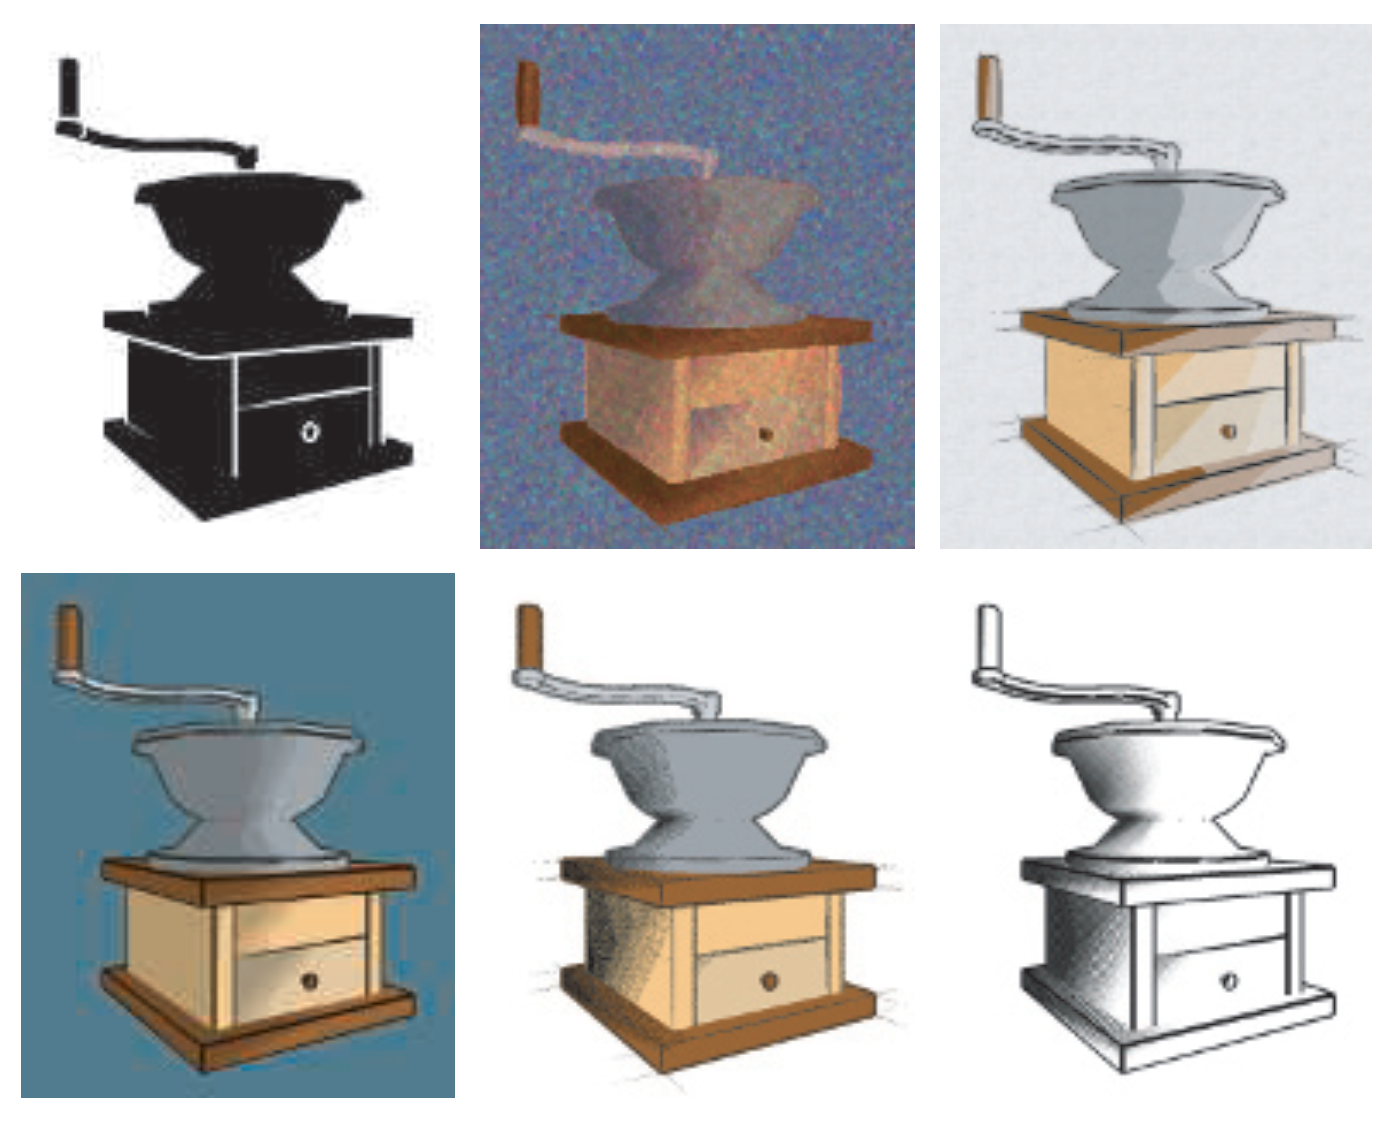
\includegraphics[width=\linewidth]{npr}
    \caption{\label{fig:npr}
    使用不同的艺术风格对一个咖啡机模型进行非真实感绘制}
\end{figure}

\begin{figure}[!b]
    \centering
    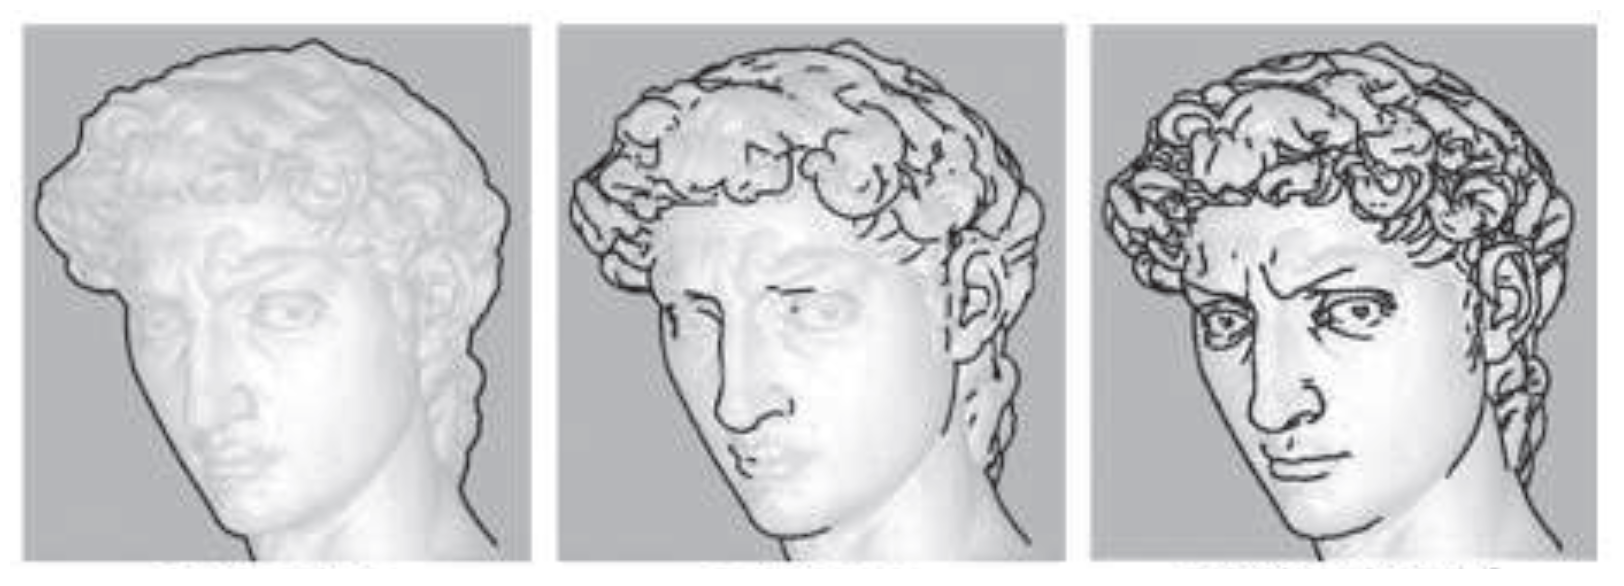
\includegraphics[width=\linewidth]{npr_lines}
    \caption{\label{fig:npr_lines}
    从左到右:外轮廓线,\con{},以及\con{}加上\scon{}的结果}
\end{figure}

就图像表现而言,实时绘制技术可以分为真实感绘制(photorealistic rendering)和\npr{}(non-photorealistic rendering)两个不同的方向。真实感绘制追求与现实世界一致的图像表现,使得用户在计算机生成的虚拟图像上体会到真实感。与之相反,\npr{}技术生成的图像与现实世界相差甚远。\npr{}旨在表现特定的卡通或简约的艺术风格,因而又称为风格化绘制(stylized rendering),来自\cite{akenine2018real}的\autoref{fig:npr}展示了一个对三维模型进行不同风格的非真实感绘制的例子。具体而言,\npr{}主要包含两个方面的技术:风格化着色(stylized shading)和线绘制(line rendering)。风格化着色旨在通过设计着色方式来表现特定的艺术风格,例如卡通着色和铅笔画风格着色。而线绘制旨在通过绘制线条来达到强调物体轮廓或简化物体外表的效果,该技术往往和不同的风格化着色搭配使用,是\npr{}中最为常用也是研究最多的一项技术。线绘制包含对各式各样的线条进行绘制的技术,例如外轮廓线(silhouette),\con{}(contour),以及\scon{}(suggestive contour)。来自\cite{akenine2018real}的\autoref{fig:npr_lines}展示了这三种线绘制技术中讨论较多的线条。本文将针对线绘制中的\con{}绘制和\scon{}绘制进行探讨。出于行文简洁的考虑,下文将三维模型表面上组成\con{}和\scon{}的点称为轮廓点,同样地,将组成\vdl{}的点成为\vdp{}。

\begin{figure}[!t]
    \centering
    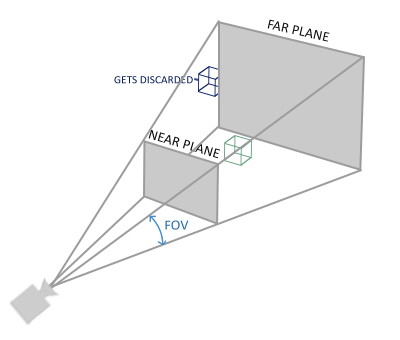
\includegraphics[width=0.6\linewidth]{view}
    \caption{\label{fig:view}
    视锥体}
\end{figure}

\begin{figure}[!b]
    \centering
    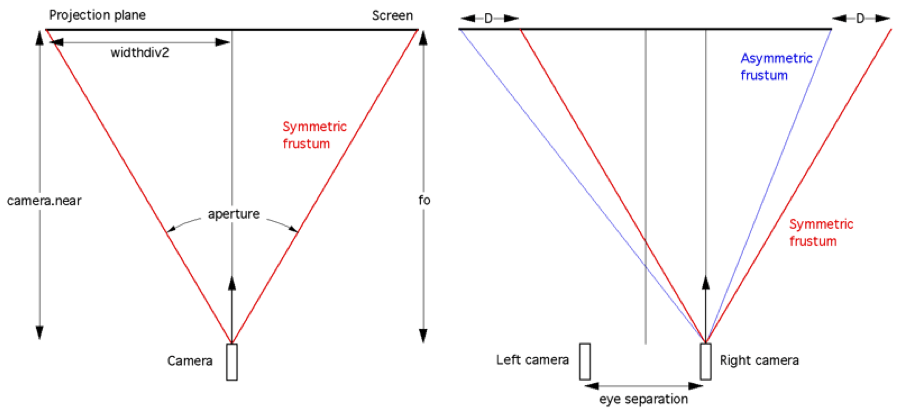
\includegraphics[width=\linewidth]{stereo}
    \caption{\label{fig:stereo}
    单目绘制和双目绘制的区别}
\end{figure}

就交互形式而言,实时绘制技术又可以分为单目绘制(monoscopic rendering)和双目绘制(stereoscopic rendering),二者的区别在于视点(viewpoint)的数目。视点是图形绘制系统中很重要的构成部分,它和光源、场景一起决定了最终绘制得到的画面。视点定义了绘制所得画面的观察位置和角度。具体而言,每个视点对应了一个视锥体(view frustum),绘制场景中只有位于视锥体内的物体部分会参与绘制并影响最终得到的画面。来自\cite{learnopengl}的\autoref{fig:view}中展示了常见的视锥体的结构。
一般而言,图形程序只需要绘制单个视点所观察的图像,即单目绘制。而对于提供三维立体感的应用,则需要绘制两个对应于双眼的视点所观察的图像从而模拟立体视觉,即双目绘制。来自\cite{topicsinopengl}的\autoref{fig:stereo}展示了单目绘制和双目绘制在视点以及视锥体上的区别。显然,由于需要对两个不同的视点进行绘制,双目绘制所需要的计算量相比于单目绘制更高,实现实时的双目绘制比起一般的实时绘制更有挑战性。尽管GPU的计算性能随着硬件技术的发展而逐年提升,但实现实时的双目绘制仍然并非易事。再者,双目绘制对于图像的质量有着更高的要求。就\con{}的双目绘制而言,如果只是直接地分别以两眼为视点分别进行绘制,绘制得到的轮廓线将不满足\stcy{}。而如果不能满足\stcy{}的要求,将会严重影响用户的体验甚至造成用户不适。因此,如何快速并正确地对\con{}进行双目绘制,是一个非常有研究价值的问题。

\begin{figure}[!t]
    \centering
    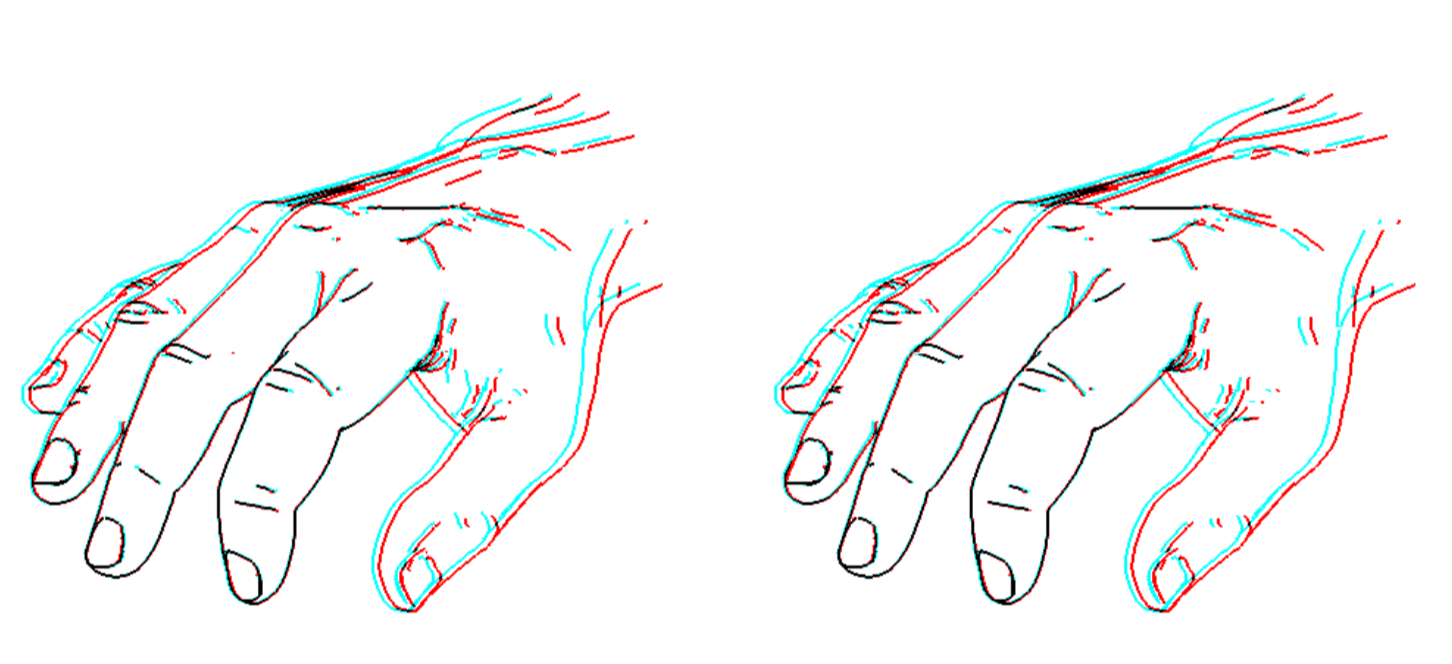
\includegraphics[width=\linewidth]{hands}
    \caption{\label{fig:hands}
    左:直接对两眼分别进行绘制,右:\stc{}轮廓线}
\end{figure}

\citeauthor{kim2013stereoscopic}在此前提出了一个\stc{}线绘制方法\cite{kim2013stereoscopic},该方法通过消除那些在另一个视点中没有对应点的\vdp{}来保证\stcy{},\autoref{fig:hands}是他们的文章中给出的对比结果。该方法的核心在于:采样多个两眼之间的视点位置绘制出多张图像,接着判定\vdp{}在这些图像中的连续性。该方法能够实现\stc{}\vdl{}绘制,但是对于复杂的物体表面而言,需要采样大量的视点来减少匹配的错误。因此,该方法需要较长的计算时间,不适用于实时绘制类型的应用。

\section{研究内容与贡献}

本文提出了一种对\stc{}(stereo-consistent)\con{}进行实时绘制的方法。在\citeauthor{kim2013stereoscopic}的工作的基础上,本文设计了一种图像空间的搜索算法来验证\conp{}的\epsl{}(epipolar-slidability)。本文方法的出发点在于:对于每个位于\ec{}(epipolar-curve)上的表面点,有一个对应的位于两眼连线上的一个视点将该表面点视为\conp{}。在此出发点的基础上,我们可以将\epsl{}的判定转换为检查这些\conp{}的对应视点的轨迹。当这些轨迹是单调地从左眼移动到右眼,或者单调地从右眼移动到左眼,那么其对应的\conp{}是\epslb{}(epipolar-slidable)的。接着,只需要去检查这些轨迹上的极值点便可判定其单调性。这个过程可以在图像空间中一次过完成,而不需要像之前的方法一样对多个视点进行采样,因而节省了大量的计算时间。这个检查对应视点的轨迹的方法对\con{}和\scon{}都适用,只是对于\scon{}而言,除了轨迹的极值点之外还需要检查轨迹的区间端点。另外,为了避免因为\conp{}或\sconp{}的重叠而导致的匹配错误,本文设计的方法使用了GPU上的\ppll{}\cite{yang2010real}来保存位于同一像素位置上的多个点的信息。实验结果表明本文提出的方法所需要的计算耗时远小于现有的方法,因而该方法能够用于实时绘制的应用中,并且支持用户对\stc{}\con{}和\scon{}的编辑,例如改变视点位置、修改物体的几何结构、调整\con{}和\scon{}的参数从而展示不同的细节等。

本文的工作主要有以下三个贡献:

\begin{itemize}
    \item 在\epsl{}的基础上作进一步的数学推导,证明\ec{}上的\conp{}和\sconp{}的\stcy{}可以通过对应视点轨迹的极值点来进行判定;
    \item 提出了一个图像空间的搜索算法,该算法可用于判定双目绘制中\con{}和\scon{}的\epsl{};
    \item 提出了一个\stc{}\con{}和\scon{}的绘制方法,该方法能够以实时的效率处理\con{}和\scon{},并且支持线条的风格化绘制。
\end{itemize}

\section{本文结构安排}

本文围绕提出的\stc{}\con{}和\scon{}的实时绘制方法进行了核心概念的理论推导以及算法设计的细致说明,全文结构安排如下:

\begin{itemize}
    \item 在第二章中介绍本文的背景知识,并介绍一些其他的相关工作;
    \item 在第三章中介绍用于单目绘制的\con{}和\scon{}的绘制方法,并且介绍线条的风格化绘制的方法;
    \item 在第四章中介绍前人提出的\epsl{}的概念,并阐述本文在\epsl{}这一概念的基础上进行的推导。
    \item 在第五章中介绍本文提出的\stc{}\con{}和\scon{}的绘制方法,并说明其中的实现细节。
    \item 在第六章中对本文提出的方法得到的结果和已有的方法得到的结果进行对比,并作分析讨论。
    \item 在第七章中对全文内容进行总结,并描述对未来研究的展望。
\end{itemize}
\chapter{背景知识与相关工作}

\section{背景知识}

\subsection{线条的概念与分类}
\label{sec:diff_geo}

在一些传统的艺术效果中,例如笔墨风格和技术说明书风格,线条的绘制是很重要的一部分。为了实现这类艺术效果,计算机图形学的研究者们提出了多种不同的算法来实现基于三维模型的线绘制。根据视点相关性,可以将线绘制所讨论的线条类型分为\vdl{}(view-dependent lines)和\vidl{}(view-independent lines)两种。

本文主要讨论的\con{}和\scon{}都属于\vdl{}。在\vdl{}中,\con{}和\scon{}是最为常用的线条类型。简单来说,\con{}表示的就是几何物体的外形的凸出部分所形成的线条。在计算机图形学领域中,常用的三维模型由三角形网格构成。具体地,\con{}就是由三维模型上视线方向和表面法线的点积为零的点所组成的线。\scon{}也是一种\vdl{},它是对\con{}的补充和视觉上的延伸。

\vidl{}也是表现几何体表面的重要特征,与\vdl{}不同的是,\vidl{}只与三维模型本身的几何性质有关。计算机图形学的研究者们已经提出了各种各样的\vdl{},例如\citeauthor{ohtake2004ridge}提出的\cite{ohtake2004ridge}岭线(ridge)和谷线(valley)和\citeauthor{yoshizawa2005fast}提出的峰线(crest)\cite{yoshizawa2005fast}。三维模型表面的折痕和模型与模型之间相交形成的交线也属于\vidl{}。由于\vidl{}和视点无关,所以它们自然是\stc{},因此本文不会对它们进行进一步的讨论。

\subsection{轮廓线的数学定义}

为了对三维模型表面的线条作出严格的、公式化的定义,计算机图形学的研究者们使用了微分几何领域的数学语言来对线条的定义进行表述。顾名思义,这个领域涉及到对曲线和表面的“微分”。对于一般的图形学研究者而言,表面法线(normal)这个概念并不陌生,它用于表示垂直于某平面的方向,广泛地用于各种绘制模型的公式之中。从微分几何的角度来看,法线其实就是表面的一阶微分。正如上一小节所述,\con{}的出现决定于法线和视线的点积是否为零。假设$N$表示表面法线,$V$表示视线方向,\con{}的决定条件即为$N\cdot{V} = 0$。类似地,其他各式各样的线条,例如\scon{},也有着和表面微分相关的数学定义,不过与之相关的是更加高阶的表面微分。

\begin{figure}[tbh]
    \centering
    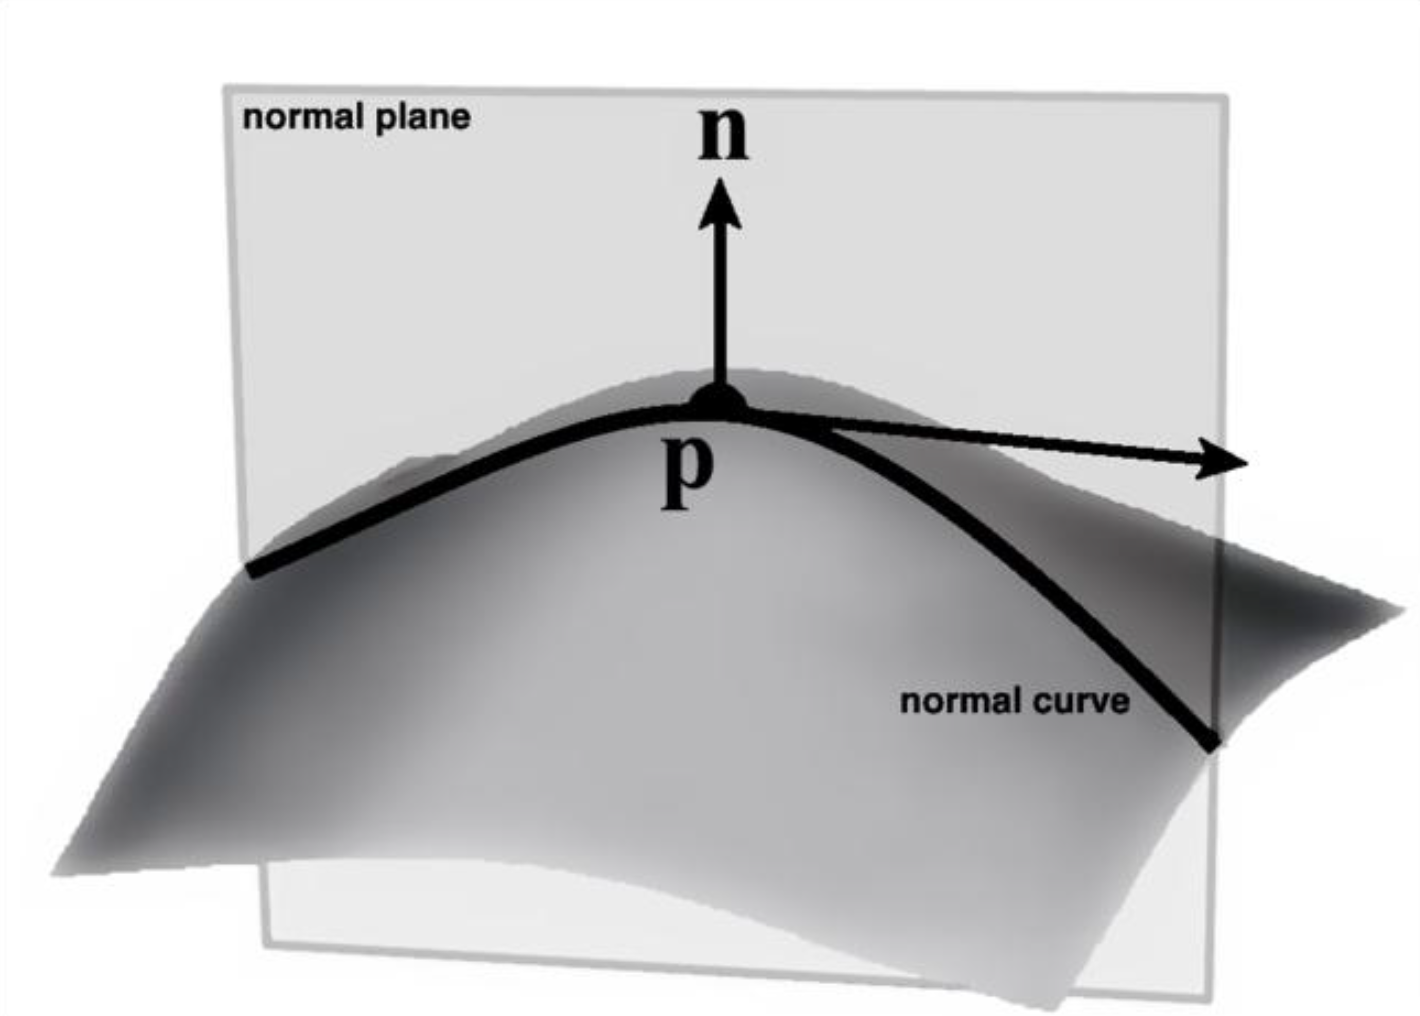
\includegraphics[width=0.6\linewidth]{normal_curvature}
    \caption{\label{fig:normal_curvature}
    法向曲线与法向曲率}
\end{figure}

简单来说,三维模型表面的二阶微分其实就是表面对应的曲率。一般常见的曲率定义与曲线相关,它表示曲线上某一点处最逼近曲线变化的圆的半径的倒数。曲线越是弯曲,曲率的值越高。对于表面而言,可以通过用包含法线的任意平面与之相交得到一条曲线,称为法向曲线(normal curve),而对应于法向曲线的曲率便是法向曲率(normal curvature)。\autoref{fig:normal_curvature}\cite{rusinkiewicz2008line}展示了法向曲率的一个例子。对于表面上的每个点,都存在多个不同的曲率,每个曲率对应于形成法向曲线所用的不同的包含该法线的平面。

\begin{figure}[tbh]
    \centering
    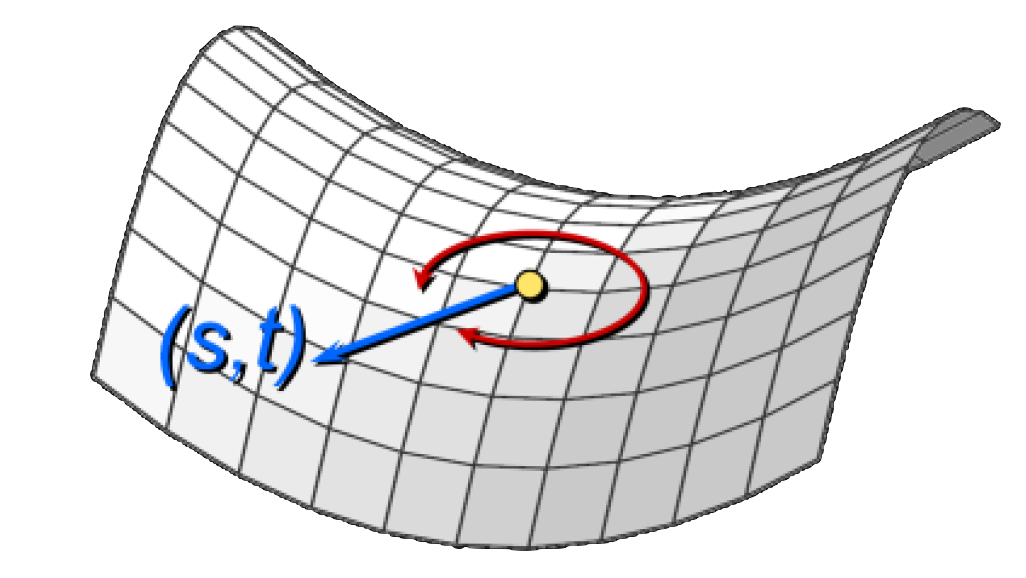
\includegraphics[width=0.6\linewidth]{sym_mat}
    \caption{\label{fig:sym_mat}
    某个方向上的法向曲率}
\end{figure}

对于一个平滑的表面,法向曲率及其对应方向的变化不是随机的,可以用一个特定的公式表示。如\autoref{fig:sym_mat}\cite{rusinkiewicz2008line}所示,假设以表面上某点的切平面建立局部的正交坐标系,对于平面上的每个方向$(s,t)$,可以找到该方向上对应的法线曲率,其表达形式与一个对称矩阵$\rm II$有关:

\begin{equation}
    \begin{split}
        \kappa_r &= 
        \begin{pmatrix}
            s & t
        \end{pmatrix}
        \begin{pmatrix}
            e & f \\
            f & g
        \end{pmatrix}
        \begin{pmatrix}
            s \\
            t
        \end{pmatrix} \\
        &= 
        \begin{pmatrix}
            s & t
        \end{pmatrix}
        \rm II
        \begin{pmatrix}
            s \\
            t
        \end{pmatrix} \\
        &= 
        \rm II((s, t), (s, t))
    \end{split}
\end{equation}

矩阵$\rm II$表达了表面的弯曲程度。在大多数的讨论中,为了简单起见,会将局部坐标系旋转使得$\rm II$是一个对角矩阵,而新的坐标轴则是$\rm II$的特征向量。

\begin{equation}
    \rm II = R^T
    \begin{pmatrix}
        \kappa_1 & 0 \\
        0 & \kappa_2
    \end{pmatrix}
    R
\end{equation}

\begin{figure}[tbh]
    \centering
    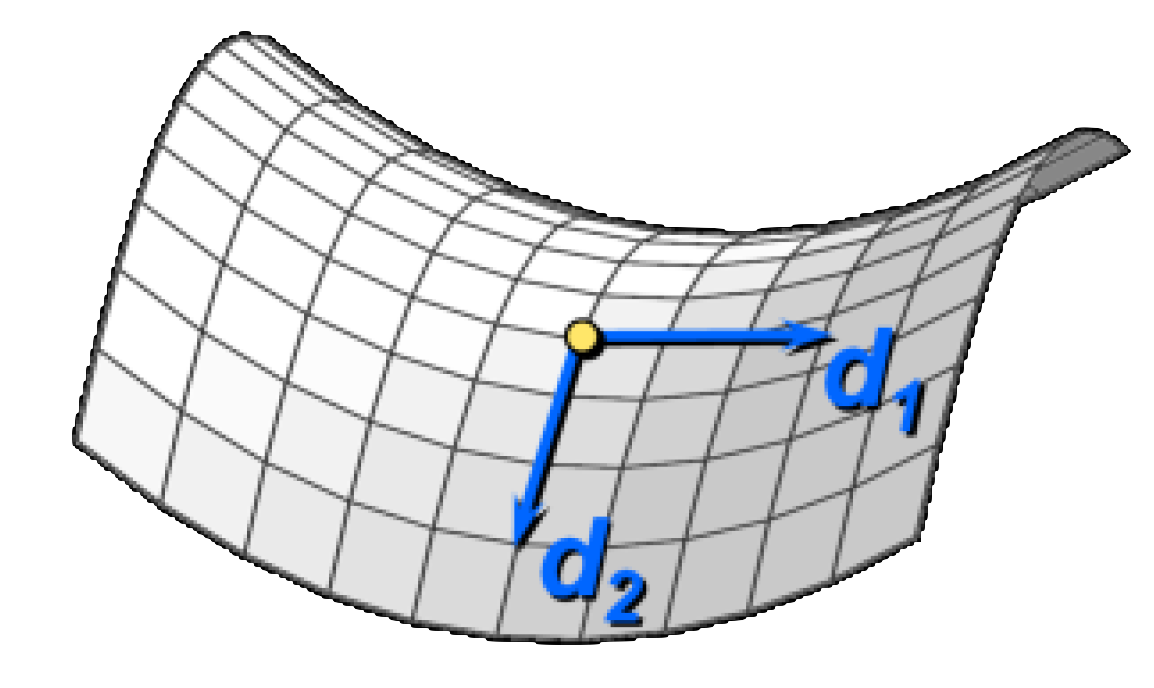
\includegraphics[width=0.6\linewidth]{sym_mat2}
    \caption{\label{fig:sym_mat2}
    主方向与主曲率}
\end{figure}

如\autoref{fig:sym_mat2}\cite{rusinkiewicz2008line}所示,在完成坐标系的转换后,新的坐标轴被称为主方向(principal direction),对应方向上的曲率被称为主曲率(principal curvature)。按照对应曲率的大小,两个主曲率又可以分别称为最小曲率和最大曲率,因为经过该点的所有曲率的值的大小都会在两个主曲率的值之间。具体而言,该点上沿着表面某个切线方向的法向曲率可以表示为:

\begin{equation}
    \kappa_r = \kappa_1\cos^2\phi + \kappa_2\sin^2\phi
\end{equation}

\begin{figure}[tbp]
    \centering
    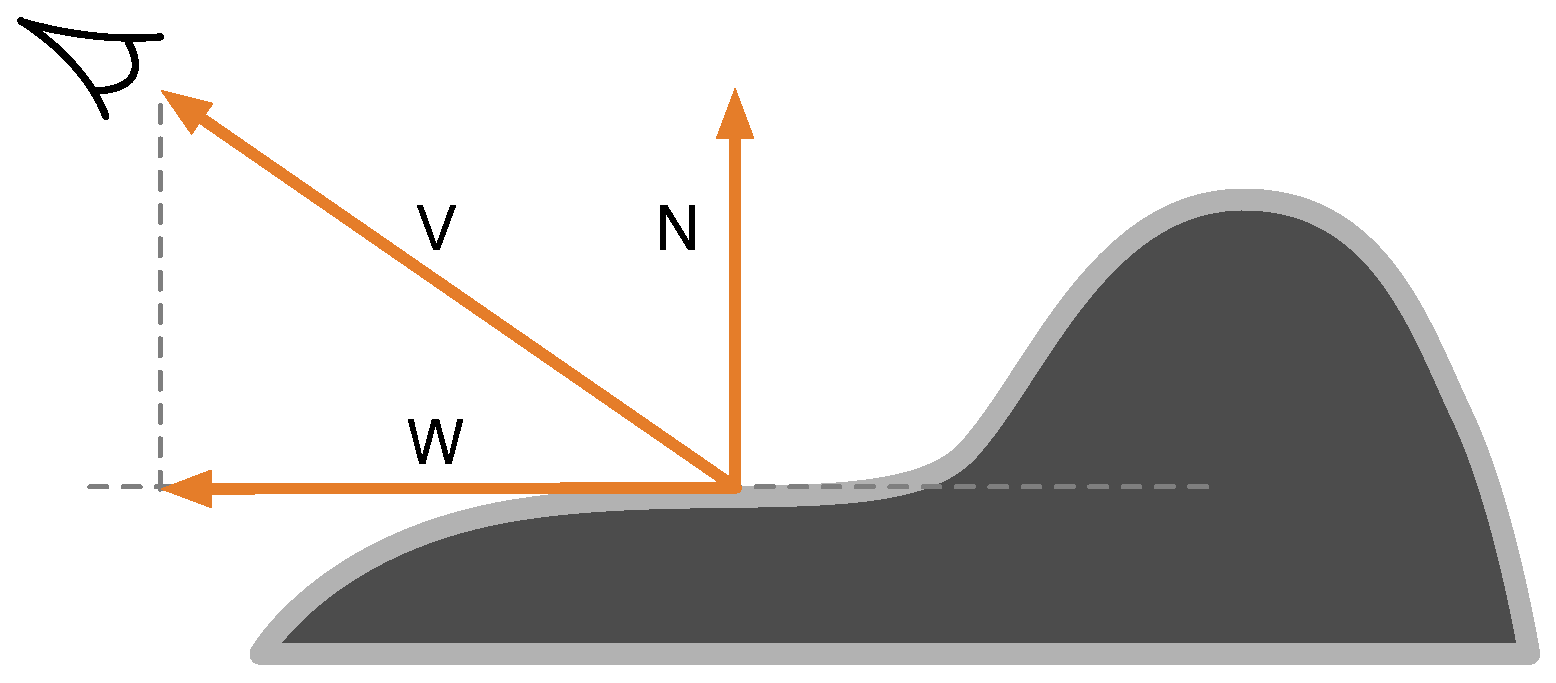
\includegraphics[width=0.8\linewidth]{suggestive_contour_definition}
    \caption{\label{fig:suggestive_contour_definition}
    \scon{}的定义。其中$N$表示表面法线,$V$表示视线方向,$W$表示$V$在切平面上的投影。}
\end{figure}

其中$\phi$表示绕主方向$d_1$转过的角度。该公式也被称为法线曲率的欧拉公式,它表示了任意方向上的曲率是关于两个主曲率的一个函数。\scon{}的定义和法向曲率直接相关。从比较直观的角度来看,\scon{}表示三维模型表面上$N\cdot{V}$在$W$方向上的局部最小值,其中$W$表示$V$在切平面的投影,\autoref{fig:suggestive_contour_definition}展示了表面上某点属于\scon{}的一个例子。换言之,要找到\scon{},其实就是要找到$N\cdot{V}$的导数的零点,并且保证此处的二阶导数的值为正。而$N\cdot{V}$在$W$方向上的导数等于$W$方向上的法向曲率$\kappa_r$乘以一个常数,推导如下:

\begin{align}
    D_w(N\cdot(V)) &= D_w{N}\cdot{V} + N\cdot{D_w{V}} \\
                   &= D_w{N}\cdot{W} \\
                   &= \rm II(W, W) \\
                   &= (W\cdot{W})\kappa_r
\end{align}
  
在上述推导中,第一行是使用链式法则展开的结果,其中第一个项中的$D_w{N}$表示$N$在$W$上的导数,它的方向必然是在切平面上,所以可以把$D_w{N}\cdot{V}$替换为$D_w{N}\cdot{W}$,而第二项中的$D_w{V}$也必然垂直于$N$,因此直接消去。所以,从公式的角度,\scon{}的定义如下:

\begin{align}
  \kappa_r &= 0\\
  D_w\kappa_r &> 0
\end{align}

其中,$W$方向上的$\kappa_r$也被称为表面上一点的径向曲率(radial curvature)。$D_w\kappa_r$表示$\kappa_r$在方向$W$上的导数,由于需要保证是局部极小值,所以需要保证二阶导数大于零。类似地,$D_w\kappa_r$可以表示为关于$W$的形式:

\begin{equation}
    D_w\kappa_r = C(W, W, W)
\end{equation}

其中$C$是一个对称的三阶张量,可以用4个常数来表示。

\section{相关工作}

\subsection{轮廓线的绘制算法}

在计算机图形学领域,研究者们针对不同的应用提出了多种多样的轮廓线绘制算法。大致地,可以将目前常用的轮廓线绘制算法分为两类,一类是基于图像处理的绘制算法,另一类是轮廓线直接检测的绘制算法。
% 已有的轮廓线的绘制算法可以大致分为四类,分别是表面角轮廓线,过程式几何轮廓线,基于图像处理的轮廓线以及轮廓线检测。

% 表面角轮廓线算法由\citeauthor{gooch1999interactive}在\cite{gooch1999interactive}中提出。该算法的核心是计算视角到表面的方向以及表面法向的点积,如果这个值接近0,那么说明这部分接近轮廓。\citeauthor{marshall2001cartoon}\cite{marshall2001cartoon}则在顶点着色器中完成部分计算,并用点积来索引一个一维纹理来实现轮廓线与其他部分的渐变。而\citeauthor{everitt2002one}在\cite{everitt2002one}中提出用纹理层级金字塔来进行这一步计算,将最顶层渲染成黑色来表现轮廓。这种做法适用于一些模型,但是对于例如正方体这类表面平滑的模型就会失败。因为在正方体某个面的法向是一致的,所以整个面的点积结果相同,会出现整个面都睡黑色或者整个面都是白色的情况。

% 最早的实时轮廓线渲染算法由\citeauthor{rossignac1992hidden}\cite{rossignac1992hidden}提出,属于过程式几何轮廓线的做法。其中的基本想法是用两遍渲染,第一遍先渲染正向视角的面,然后以某种方式渲染背向视角的面并使它们突出正向面一部分,最终达到轮廓线的效果。有数种不同的方法来渲染背向的平面,可以增加背向面的深度值使其突出,或者直接使背向面向摄像机位置移动,还可以对背向面的三角形面片进行放大,Raskar和Cohen在他们的工作\cite{raskar1999image}中研究了这些做法。无论以哪一种做法突出背向面,都有轮廓线的大小难以统一调控的问题,不便于进行风格化渲染。

基于图像处理的轮廓线绘制算法实现起来较为简单直接,其核心思想是利用G缓冲(G-buffer)中存储的信息在图像空间判断是否出现轮廓线。G缓冲是延迟着色\cite{duluk2004deferred}的绘制流程的中间产物。在延迟着色的第一个阶段中,场景会被绘制一次但不进行着色,只是将三维模型的位置、法向等信息存储到一个图像空间的缓冲中,这个缓冲被成为G缓冲。在延迟着色的第二个阶段,再通过一个全屏后处理以G缓冲作为输入完成着色。\citeauthor{decaudin1996cartoon}拓展了G缓冲的使用方法,在他们的工作\cite{decaudin1996cartoon}中,以G缓冲中的法线和深度信息组成输入,利用索贝尔算子\cite{gao2010improved}等图像滤波的方法进行边缘检测,从而绘制出轮廓线。基于图像处理的方法的好处在于适用性强,只需要一个全屏后处理即可完成,而且可以同时在后处理中完成其他类型的线条的绘制,在效率上有着很大的优势。但是,在绘制质量上,基于图像处理的方法并不占优。该方法的缺陷在于:在深度变化较小或者法线变化较小的区域,例如放在桌子上的纸面的边界,该方法并不能正确地绘制出轮廓线。另外,索贝尔算子等边缘检测方法大多不是良定义的,其最终效果的好坏一定程度上依赖于一些输入参数的人工调节,效果并不稳定。

% 随着延迟渲染的兴起,基于图像处理的轮廓线渲染算法也发展了起来。G-buffer是延迟渲染中的重要一环,\citeauthor{decaudin1996cartoon}\cite{decaudin1996cartoon}拓展了G-buffer的使用方法,利用其中储存的信息作为轮廓线判断的依据。该算法的核心是将图像空间的法线和深度信息组成一个4通道的缓冲,利用索贝尔算子\cite{gao2010improved}等滤波方法进行边缘检测。好处在于适用性强,直接在GPU端可以完成,而且会将轮廓边和其他类型的边界一同检测出来进行所需的渲染,同时省去了轮廓线可见性的检测。该算法的缺陷相对来说比较小,在深度变化小或者法向变化小的地方会失败,例如放在桌子上的纸面的轮廓就无法检测出来。

相比于基于图像处理的轮廓线绘制算法存在上述的各种缺点,而轮廓线的直接检测的绘制算法在绘制质量以及可控性上明显要更好一些。轮廓线的直接检测指的是在世界空间或对象空间直接根据三维模型的几何信息检测出轮廓线,这一类绘制算法能够对线条进行更加精细的操作,方便对线条进行进一步的风格化绘制。轮廓线的直接检测较早的做法\cite{marshall2001cartoon}是遍历三维模型的三角形网格上的每一条边,判断这些边是否属于轮廓线并保存对应的信息。尽管可以通过排除同一个面的边或者保存每个面的点积等方法来进行优化,但是由于每一帧都要对于新的视点重新遍历三角形网格,这种方法的计算耗时依然很大。\citeauthor{decaudin1996cartoon}提出来一个更高效的做法\cite{decaudin1996cartoon}。他们的核心想法是,假设帧与帧之间视点和物体之间发生的移动较少,可以认为上一帧检测的轮廓线在这一帧依然会是轮廓线。他们通过计算上述的移动距离从而避免每一帧的重新遍历所需的计算量,相较于前者的方法在效率上获得来很大的提升。由于检测过程中可以精确地获取轮廓线的信息,轮廓线的直接检测对进一步的风格化处理非常有利,但是相较于基于图像处理的方法而言,实现上较为复杂。不过,随着现代GPU绘制流水线的发展,可编程着色器越来越灵活,轮廓线的直接检测方法也可以实现地非常简单而又高效。目前比较高效的实现方法是使用可编程着色器中的几何着色器(geometry shader)来完成轮廓线的直接检测,这样可以充分利用GPU的并行计算的高性能,并摆脱传统方法中CPU与GPU的交互,直接在绘制流水线中完成轮廓线的绘制,使得绘制效率大大提升。本文正是通过编写几何着色器来高效地实现\con{}以及\scon{}的绘制算法,在下文的第二章中会进行相关的具体说明。

% 以上介绍的方法大多有着需要两遍渲染的缺点,而且不便于对轮廓边进行风格化渲染。轮廓线的直接检测指的是在对象空间检测出轮廓线,该算法能够对渲染线进行更加精细的操作。轮廓线的直接检测的标准做法是遍历三角形网格中的每一条边,检测出所有的轮廓边并保存对应的信息\cite{marshall2001cartoon}。可以排除同一个面的边或者保存每个面的点积结果来进行优化,但是由于每次渲染都需要重新进行遍历,所以仍然会带来很大的计算成本,影响实时渲染的帧率。Hall等人提出了一个高效的优化手段\cite{decaudin1996cartoon}。假设帧与帧之间摄像机和物体的进行了较少的移动,可以认为上一帧检测的轮廓边在这一帧依然会是轮廓边。通过对移动距离的计算从而省去每一帧的大量检测计算,最终得到了成倍的性能提升。轮廓线的直接检测对进一步的风格化非常有利,缺点是高效的实现较为复杂。不过,随着现代GPU绘制流水线的发展,可编程着色器越来越灵活,轮廓线的直接检测方法也可以实现地非常高效。目前比较高效的实现方法是使用可编程着色器中的几何着色器(geometry shader)来完成轮廓线的直接检测,这样可以充分利用GPU的并行计算的高性能,并摆脱传统方法中CPU与GPU的交互,直接在绘制流水线中完成轮廓线的绘制,使得绘制效率大大提升。本文正是通过编写几何着色器来高效地实现\con{}以及\scon{}的绘制算法,在下文的第二章中会进行相关的具体说明。

\begin{figure}[tbh]
    \centering
    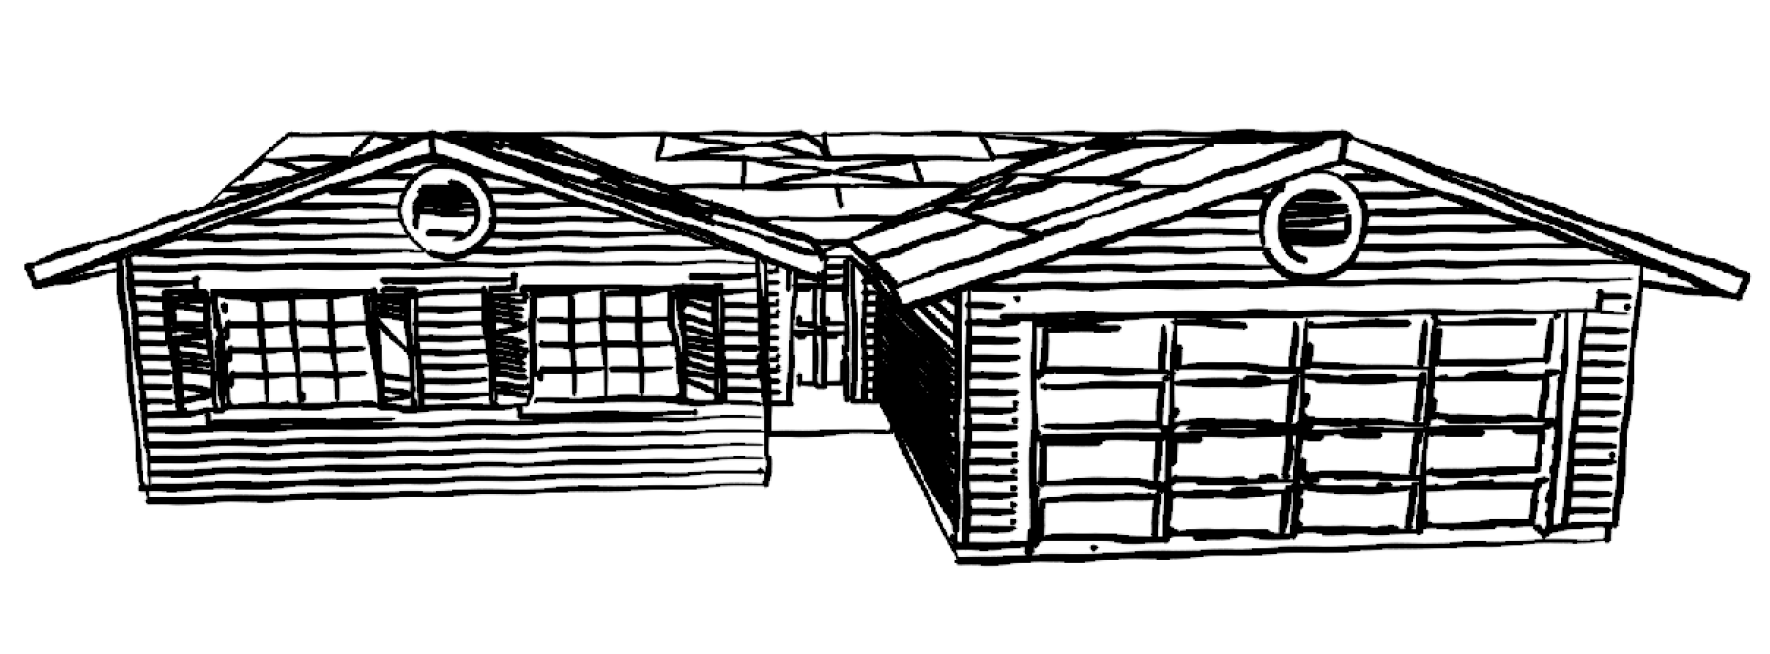
\includegraphics[width=\linewidth]{stylized_house}
    \caption{\label{fig:stylized_house}
    使用风格化线条绘制的建筑物}
\end{figure}

需要特别指出的是,虽然线绘制本身属于非真实感绘制或者风格化绘制的其中一种技术,但是关于线条的进一步风格化也是一项独立的研究课题:风格化线条(stylized line)。一般的线绘制只是涉及如何利用绘制流水线构建给定定义的线条并进行快速的绘制,而风格化线条指的是在此基础上对线条的外形、着色进行艺术风格的表达,例如使线条呈现出毛笔、笔刷等绘画工具的质感。来自\cite{northrup2000artistic}的\autoref{fig:stylized_house}展示了风格化线条的一个例子。\citeauthor{northrup2000artistic}在\cite{northrup2000artistic}中提出了对轮廓线进行进一步风格化的方法。在他们的方法中,先按照已有的方法找到所有轮廓线的线段,然后处理这些线段之间的重叠并将在图像空间线段连接成连续的长线。接着,再以这些长线为对象进行绘制,在绘制的过程中将线条沿着法线方向展开为四边形,使得最后在着色阶段可以贴上纹理进行绘制,进而表现出特定的笔刷效果。\citeauthor{isenberg2002stylizing}在\cite{isenberg2002stylizing}中提出了改进的方法。在前人的方法中,线段之间是通过在图像空间搜索相邻的端点来建立连接的,而\citeauthor{isenberg2002stylizing}的方法将这一步骤改进为利用三维模型本身的三角形的邻接关系来寻找相邻的端点,使得绘制速度获得了很大的提升。

\subsection{\stc{}\npr{}}

线绘制属于\npr{}技术中的一种。一般而言,\npr{}的相关研究只关注如何解决单目绘制下的问题。不过,近年来\npr{}和双目绘制的结合越来越受到关注,出现了不少关于\npr{}在双目绘制下的问题的研究。为了避免双目绘制下基于笔画的图像风格化算法\cite{hertzmann1998painterly}带来的问题,\citeauthor{northam2012consistent}\cite{northam2012consistent,northam2013stereoscopic}提出了将左眼和右眼的画面分离成离散的差异层的方法。在得到左眼和右眼对应的差异层后,他们提出的方法将对应的层组合起来再作进一步的基于笔画的风格化,从而得到\stc{}的图像。\autoref{fig:disparity}展示了用他们提出的方法得到的一个结果。

\begin{figure}[tbh]
    \centering
    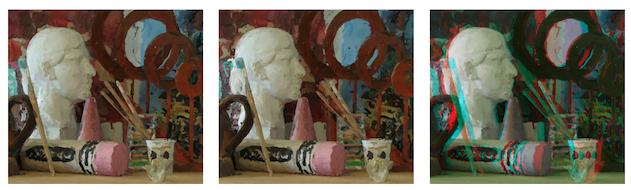
\includegraphics[width=\linewidth]{disparity}
    \caption{\label{fig:disparity}
    立体一致的基于笔画的图像风格化}
\end{figure}

除了基于图像的风格化算法,基于三维模型的线绘制在双目绘制下的问题也有一定的研究。\citeauthor{kim2013stereoscopic}在他们的工作中具体定义了关于轮廓线的\stc{}概念,并提出了在多个视点上检查对极曲线上的对应轮廓点的的方法来保证轮廓线的立体一致性,该方法对于\scon{}也同样适用。此外,\citeauthor{bukenberger2018stereo}在近年提出了一个新的方法\cite{bukenberger2018stereo}来解决\stc{}\vdl{}绘制这个问题。与前者在图像空间中处理的方法相比,他们的方法着力于利用物体空间的信息来解决这个问题。他们的方法首先绘制出不同给定视点下的\vdl{}的结果并以物体空间的形式存储下来,接着利用这些信息通过插值得出新视点下立体一致的\vdl{}的图像。

在\stc{}\vdl{}绘制的基础上,如何做进一步的风格化的问题也得到了关注\cite{northrup2000artistic,kalnins2003coherent} 。\citeauthor{kim2013stereoscopic}和\citeauthor{bukenberger2018stereo}都在他们各自的工作中提出了对\stc{}的\vdl{}进行风格化的方法。在获得不同视点下轮廓点的对应关系的基础上,\citeauthor{kim2013stereoscopic}在不同视点之间传递风格化参数的方法,从而保证进一步的风格化处理依然保持最后结果是\stc{}。在\citeauthor{bukenberger2018stereo}的工作中,进一步的风格化参数由物体的三维表面的一些特征决定,以此来保证结果的时序一致性(temporal coherency)。同样,本文将先就如何实现\stc{}\con{}和\scon{}来进行阐述,然后再描述进一步风格化的解决方法。

\subsection{\ppll{}}

\begin{figure}[tbh]
    \centering
    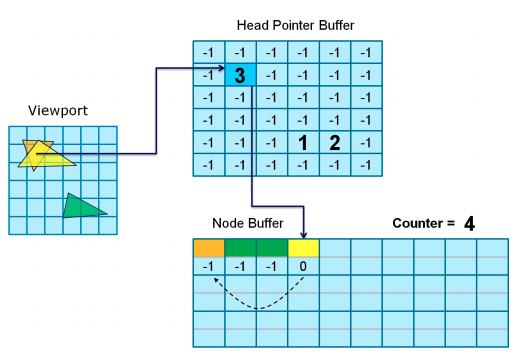
\includegraphics[width=\linewidth]{ppll}
    \caption{\label{fig:ppll}
    \ppll{}所使用的数据结构}
\end{figure}

链表是计算机领域中常用的一种数据结构。链表往往用于存储不定长度的数据集合,在各式各样的CPU上的算法上很常见也易于实现,但是在GPU上没有简单直接的实现方法。\citeauthor{yang2010real}提出了一个高效的方法\cite{yang2010real}来在GPU上构建链表。他们的方法使用一个缓冲来存储所有的链表节点,并使用另一个图像空间的缓冲区来存储逐个像素上的链表头部节点,这些头部节点指向上述第一个缓冲中的用于存储实际信息的节点,\autoref{fig:ppll}展示了他们设计的数据结构。\ppll{}是用来处理逐个像素上的多个片段(fragment)的最具有普适性的工具,一个典型的用例是进行排序无关的透明绘制(order independent transparency)。在一般的绘制流程中,由于深度测试(depth test)的存在以及透明物体做透明度混合(alpha blending)的需要,往往需要在CPU端先对各个三维模型从远到近进行排序,然后按顺序进行绘制,否则会导致远处的透明物体被近处的透明物体所遮挡的错误结果。在\citeauthor{barta2011order}的工作中\cite{barta2011order},他们提出了用\ppll{}来进行排序无关的透明绘制的方法。在他们的方法中,不需要在CPU端对三维模型进行排序,而是先将三维模型绘制到\ppll{}上,其中每个像素存储了多个来自于不同的三维模型的片段颜色以及对应的距离,然后通过另外一个全屏后处理对\ppll{}上每个像素的多个片段按照距离进行排序并计算出透明度混合的结果。由于只需要在片段着色器阶段对多个片段进行排序,整个过程可以完全在GPU中实现,所以相比一般在CPU端进行排序的方法效率更高,而且更加灵活。

为了避免轮廓点的重叠带来的问题,本文设计的方法使用\ppll{}来访问位于同一个像素点上的多个不同轮廓点的数据。由于本文设计的方法只需要对轮廓点建立链表,而这些轮廓点只占整体画面的一小部分,所以\ppll{}的内存占用量并不大。
\chapter{\con{}和\scon{}绘制算法}

在讨论如何实现\stc{}\con{}和\scon{}绘制之前,本文将先对不考虑\stcy{}的\con{}和\scon{}绘制进行说明。本文所实现的\con{}和\scon{}绘制算法参考自Northrup等人和Isenberg等人的工作\cite{northrup2000artistic,isenberg2002stylizing},但在具体实现上最大化利用了现代绘制流水线提供的一些机制。考虑到后续还需要执行\stc{}相关处理,高效地实现作为基础的\con{}和\scon{}的绘制是十分有必要的。

\section{\con{}和\scon{}的直接绘制}
\label{sec:basic}

在不考虑进一步的风格化处理的情况下,本文所实现的\con{}和\scon{}的直接绘制需要进行两次绘制:

\begin{itemize}
    \item 先绘制一次场景中所有的三维模型但不进行着色,得到用于可见性测试的深度图;
    \item 再绘制一次场景中所有的三维模型,完成\con{}和\scon{}的检测,并在着色阶段采样上一次绘制得到的深度图完成可见性测试;
\end{itemize}

下文将围绕这两步进行具体的说明。

\subsection{深度图与可见性测试}

先绘制一次场景中所有的三维模型来获取深度图,再通过第二次绘制来完成深度测试并着色,这在实时绘制领域是一种常见的做法,这种做法被称为深度预绘制(z prepass)。相比于直接将场景中所有的三维模型在一次绘制过程中完成深度测试并着色,深度预绘制这种做法能够提前将被遮挡的片段剔除,避免无意义的片段着色器的计算量。

但是,本文在实现\con{}和\scon{}的绘制的过程中选择采用深度预绘制,主要并不是为了减少片段着色器的计算量。直接通过绘制一次场景中所有的三维模型亦可完成\con{}和\scon{}的检测以及着色,但无法正确完成线条的可见性测试,因为深度缓冲只会在片段着色器执行的像素上更新深度,也就意味着直接依赖深度测试的话只会出现线条与线条之间的遮挡,线条被模型的几何实体所遮挡的现象无法被正确地呈现出来。

另外,本文所采取的也不是一般的深度预绘制。在一般的深度预绘制中,片段着色器不需要执行任何的代码,绘制流水线会默认使用片段着色器传入的深度更新深度缓冲。而在本文采取的深度预绘制在片段着色器对默认的深度值加上了一定的偏差。从另一个角度看,加上偏差使得深度缓冲代表了稍远一些的三维模型的深度,保证位于三维模型表面上的线条不会被三维模型的几何实体所遮挡。类似的做法也常用于贴花(decal)的绘制。由于深度缓冲的精度有限而线条本身的深度和三维模型表面的深度又十分接近,如果不对默认的深度值进行调整,会出现本应可见的线条出现部分的断裂,整体看来十分不连续,所以给深度值加上一定的偏差是很有必要的。再者,为了进一步消除可见性的带来的不连续性,在第二次绘制中也不是直接使用深度图进行深度测试,而是在片段着色器阶段沿着线条的方向对深度图进行多次采样,统计可见样本占总样本的个数作为透明度进行混合,使得最终呈现出来的线条更加均匀且连续。

\subsection{\con{}和\scon{}的检测}

\begin{figure}[!t]
    \centering
    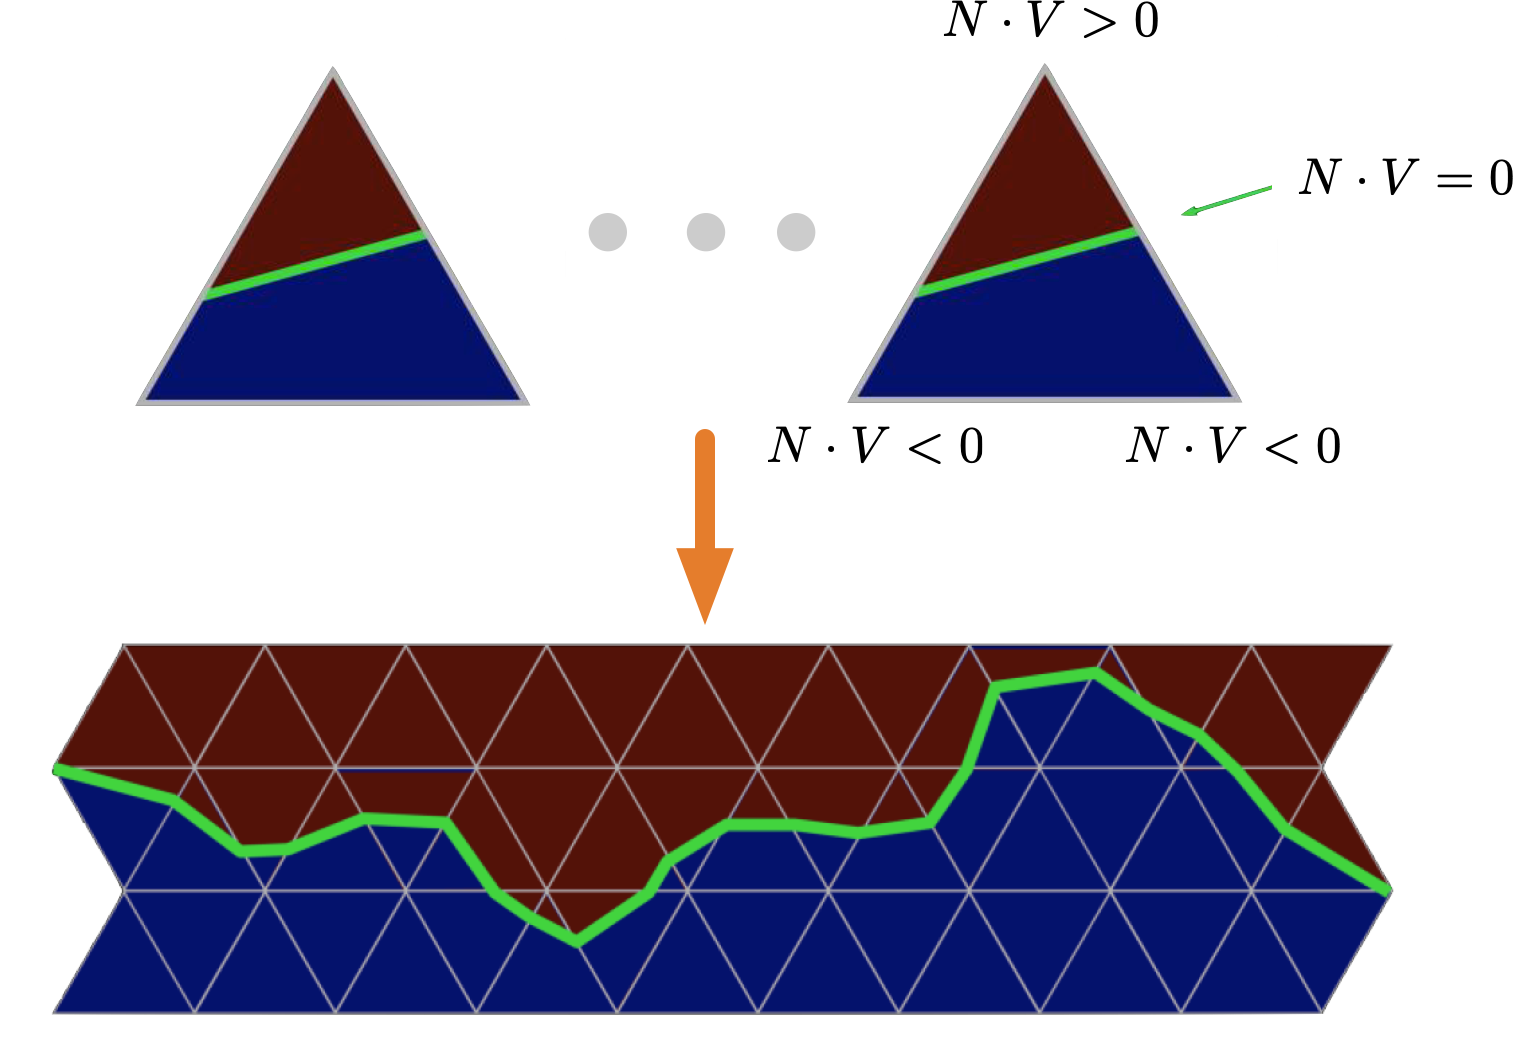
\includegraphics[width=0.8\linewidth]{detect_contours}
    \caption[轮廓线的检测]{\label{fig:detect_contours}
    上:检测三角形中的\con{}的线段,下:形成连续的长线}
\end{figure}

一般情况下,绘制流水线只涉及到顶点着色器和片段着色器的使用,其中顶点着色器负责对三维模型的顶点进行投影变换,在经过光栅化阶段后,对顶点属性进行插值并传入片段着色器进行像素上的颜色计算。几何着色器是绘制流水线中的一个可选阶段,它的执行顺序在顶点着色器和片段着色器之间。几何着色器的输入是一组顶点以及对应的顶点着色器的输出,这些顶点属于一个绘制指令指定的图元结构,可以是点、线或者三角形。以这些信息作为输入,几何着色器可以组织出新的一个或多个图元,并附上各个顶点的属性作为输出。这些新的图元会进入光栅化阶段,几何着色器输出的顶点属性也随之进入片段着色器阶段用于像素颜色的计算。

和\scon{}的检测主要使用几何着色器重新构建图元的功能来完成。具体地,绘制指令所指定的绘制对象是三维模型上的三角形,这些三角形会经过几何着色器阶段转变为代表线条的图元,最终在片段着色器阶段完成可见性检测以及着色。下面按照绘制流水线的执行顺序分别对\con{}和\scon{}的检测进行具体说明。

\textbf{\con{}的检测:} \con{}的定义为:

\begin{equation}
    N\cdot{V} = 0
\end{equation}

其中$N$表示表面法线,$V$表示视线方向。为了实现\con{}的检测,在顶点着色器阶段,除了完成一般的投影变换的计算,还要输出世界空间的法线方向和顶点位置。接着,在几何着色器阶段,分别对三角形的三个顶点计算$N\cdot{V}$的值。由于$N\cdot{V}$的值在三角形内部是连续变化的,所以可以按照如\autoref{fig:detect_contours}所示的流程来找出$N\cdot{V} = 0$的轮廓线。具体地,如果存在其中一个顶点的$N\cdot{V}$的值和其他两个顶点的$N\cdot{V}$的值异号,则判断存在轮廓线,然后分别对$N\cdot{V}$的值异号的两组顶点通过插值找到边上$N\cdot{V} = 0$的两个点,以这两个点作为端点构建线图元作为几何着色器的输出;否则不输出任何图元。

\textbf{\scon{}的检测:} \scon{}的定义为:

\begin{align}
  \kappa_r &= 0 \label{eq:Kr0} \\
  D_w\kappa_r &> 0 \label{eq:DwKr0} 
\end{align}

其中$\kappa_r$表示表面上一点的径向曲率,$D_w\kappa_r$表示$\kappa_r$的方向导数。更确切地说,$\kappa_r$是视线方向$V$在切平面上的投影$W$的方向上的法向曲率。法向曲率的概念已经在\autoref{sec:diff_geo}中进行说明,在此不再赘述。由于\scon{}的检测需要三维模型的曲率信息,而三维模型本身只记录了各个顶点的位置和法线,因此相比于\con{}的检测,\scon{}的检测需要对三维模型进行预处理来获取额外的信息。本文在实现中使用了trimesh\footnote{\url{https://gfx.cs.princeton.edu/proj/trimesh2/}}来对三维模型进行预处理得到各个顶点的主方向、主曲率以及表示曲率方向导数的张量,并将这些信息作为顶点属性传入顶点着色器阶段。

在顶点着色器阶段,首先计算出视线方向$V$在当前顶点的切平面上的投影$W$,然后计算出$W$与主方向的夹角并进一步得到当前顶点的径向曲率$\kappa_r$以及$D_w\kappa_r$。接着,在几何着色器阶段,根据三角形的三个顶点的$\kappa_r$的值通过插值找出三角形的边上存在的$\kappa_r = 0$的点。这个过程和\autoref{fig:detect_contours}所展示的过程一样,只是将$N\cdot{V}$修改为$\kappa_r$。但和\con{}的检测不同的是,为了满足\autoref{eq:DwKr0}的条件,还需要插值出$\kappa_r = 0$的点上的$D_w\kappa_r$的值,并依据$D_w\kappa_r$的值截取出$\kappa_r = 0$的两点形成的线段中$D_w\kappa_r > 0$的部分。具体地,如果两个点上的$D_w\kappa_r$的值都大于0,则保留整个线段作为输出图元;如果如果两个点上的$D_w\kappa_r$的值都小于0,则去掉整个线段,不输出图元;如果两个点上的$D_w\kappa_r$的值异号,则在这两点之间插值出$D_w\kappa_r = 0$的点,并取这个点与$D_w\kappa_r > 0$的端点组成新的线段作为输出图元。

\section{\con{}和\scon{}的风格化绘制}

如果要实现线条的风格化绘制,整体的绘制流程需要在前文描述的两次绘制的基础上进行改动。具体地,\con{}和\scon{}的风格化绘制的主要有以下几个步骤:

\begin{itemize}
    \item 先绘制一次场景中所有的三维模型但不进行着色,得到用于可见性测试的深度图;
    \item 再绘制一次场景中所有的三维模型,完成\con{}和\scon{}的检测,将检测得到的线段传到CPU端;
    \item 在CPU端对线段进行连接,并对连接后的长线进行过滤;
    \item 将处理后的长线传入GPU端以线为图元进行绘制,在绘制过程中并将长线的各个线段展开为四边形,完成可见性测试以及着色;
\end{itemize}

与直接绘制相比,线条的风格化绘制的特点在于需要将GPU端检测到的线段传递到CPU端进行处理,再传回GPU端进行绘制。尽管CPU与GPU之间相互的数据传输会造成绘制流水线的停滞,影响整体的绘制速度,但是这么做对于线条的风格化绘制来说是必要的。上述\con{}和\scon{}的直接绘制本质上是对三维模型上的各个三角形内部的\con{}和\scon{}线段并行地进行绘制,这些线段中有很大一部分会因为邻接关系连接成一条连续的长线,最终在画面上呈现出多条连续的长线。\con{}和\scon{}的直接绘制不需要关心最后连接得到的长线的具体结构(例如各个端点的位置、线段与线段之间的夹角),但是线条的风格化绘制需要获知这些信息,才能对每段连接线整体进行单独的纹理着色,保证画面上呈现出来的是连续的多条特定风格的笔画。由于目前的绘制流水线还不够灵活,无法在GPU端实现利用三角形之间的邻接关系来连接线段的逻辑,所以只能将检测得到的线段传递到CPU端进行连接。

\begin{figure}[tbh]
    \centering
    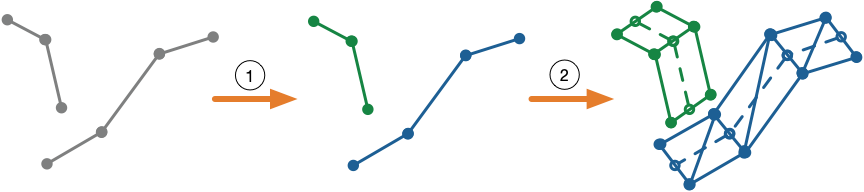
\includegraphics[width=\linewidth]{link_quad}
    \caption[线条的风格化绘制]{\label{fig:link_quad}
    1:连接邻接的线段,2:将线段拓展为四边形}
\end{figure}

接下来下文对\con{}和\scon{}的风格化绘制的步骤进行具体的说明。其中第一步与\con{}和\scon{}的直接绘制相同,在此处不再赘述。

在第二步中,本文使用了完全相同的几何着色器来完成\con{}和\scon{}的检测,但是绘制流水线就在几何着色器阶段结束,并使用变换反馈(transform feedback)\footnote{\url{https://www.khronos.org/opengl/wiki/Transform_Feedback}}的机制将几何着色器创建的线图元传递到CPU端,且每个线段附带有所在三角形的索引。

在第三步中,根据GPU端传回的线段与三角形的对应关系,以及三维模型本身带有的三角形与三角形之间的邻接关系,连接线段并构建长线。接着,遍历所有得到的长线进行过滤,如果不满足预先设定的一些条件,例如其中某条线段的长度过小、两条线段之间的夹角过大,则将长线断开。此处的过滤是为了减少长线在局部上的跳变,使得最终呈现出来的线条更加均匀连续。最后再遍历过滤后得到的每条长线,将其构建为GPU绘制所需要的数据结构,并给长线上的每个顶点附加上后续绘制需要的信息,例如随着每段线段的长度占总长度增加的纹理坐标。

在第四步中,使用绘制流水线分别对每条长线进行绘制。在顶点着色器阶段,只需完成基本的投影变换的计算。在几何着色器阶段,根据两个输入的顶点的位置信息,将其以一定的宽度展开,构建出四个新的顶点从而形成四边形,同时将原顶点的纹理坐标等属性传递到新顶点上。在几何着色器阶段的最后,以三角形作为输出图元类型,并输出组成这个四边形的两个三角形。形成四边形的目的在于给予线条一定的宽度,使得后续的纹理着色成为可能。在后续的片段着色器阶段,则可以使用传入的纹理坐标对特定艺术风格的笔画纹理进行采样,完成最终的着色。

线条的风格化绘制的核心就在于第三步的邻接线段连接以及第四步的线段到四边形的拓展,\autoref{fig:link_quad}对这两个核心步骤进行了简要的举例说明。
% \cite{kim2013stereoscopic}
% \cite{bukenberger2018stereo}
% \cite{wysiwyg2002drawing}
% \cite{geiger1995occlusions}
% \cite{cole2008people}
% \cite{rusinkiewicz2008line}
% \cite{hertzmann2000illustrating}
% \cite{raskar1999image}
% \cite{decarlo2003suggestive}
% \cite{raskar2001hardware}
% \cite{yang2010real}
% \cite{decarlo2002stylization}
% \cite{stavrakis2005image}
% \cite{hertzmann1998painterly}
% \cite{northam2012consistent}
% \cite{northam2013stereoscopic}
% \cite{northrup2000artistic}
% \cite{kalnins2003coherent}
% \cite{everitt2001interactive}
% \cite{cole2010two}
% \cite{appel1967notion}
% \cite{DFRS03}
% \cite{INR04}
\chapter{\epsl{}的概念与推导}

\begin{figure}[tbh]
    \centering
    \subfloat[\epslb{}]{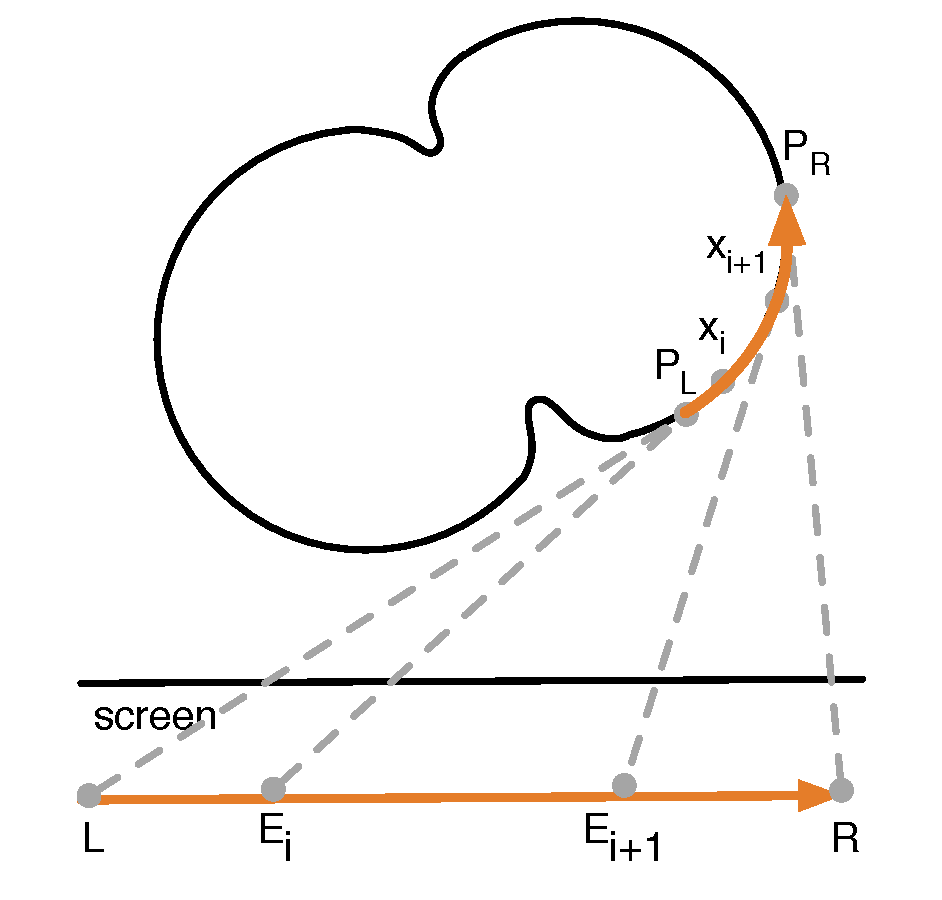
\includegraphics[width=.5\linewidth]{slidable}}
    \hfil
    \subfloat[不是\epslb{}]{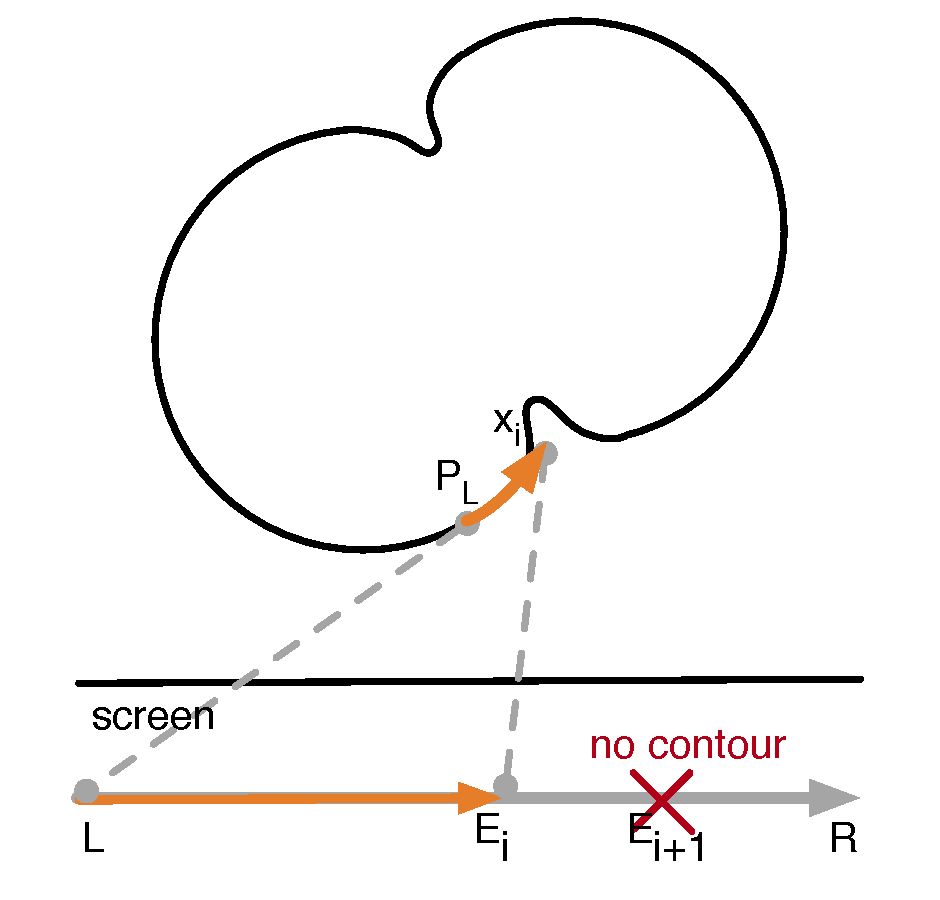
\includegraphics[width=.5\linewidth]{unslidable}}
    \caption{\epsl{}。(a)表示$P_L$是\epslb{},(b)表示$P_L$不是\epslb{}。} \label{fig_sim2}
    \label{fig:slidability}
\end{figure}

\begin{figure}[tbh]
    \centering
    \subfloat[\epslb{}]{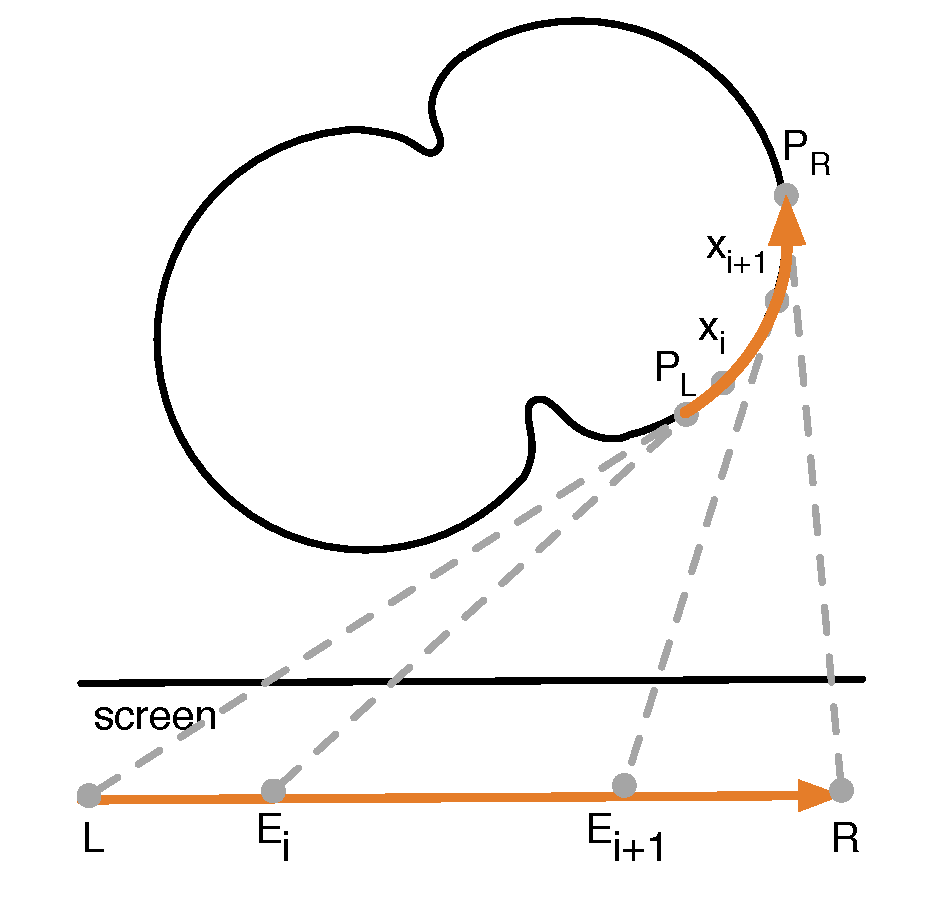
\includegraphics[width=.5\linewidth]{inverse_slidable}\label{fig:inverse_slidable}}
    \hfil
    \subfloat[不是\epslb{}]{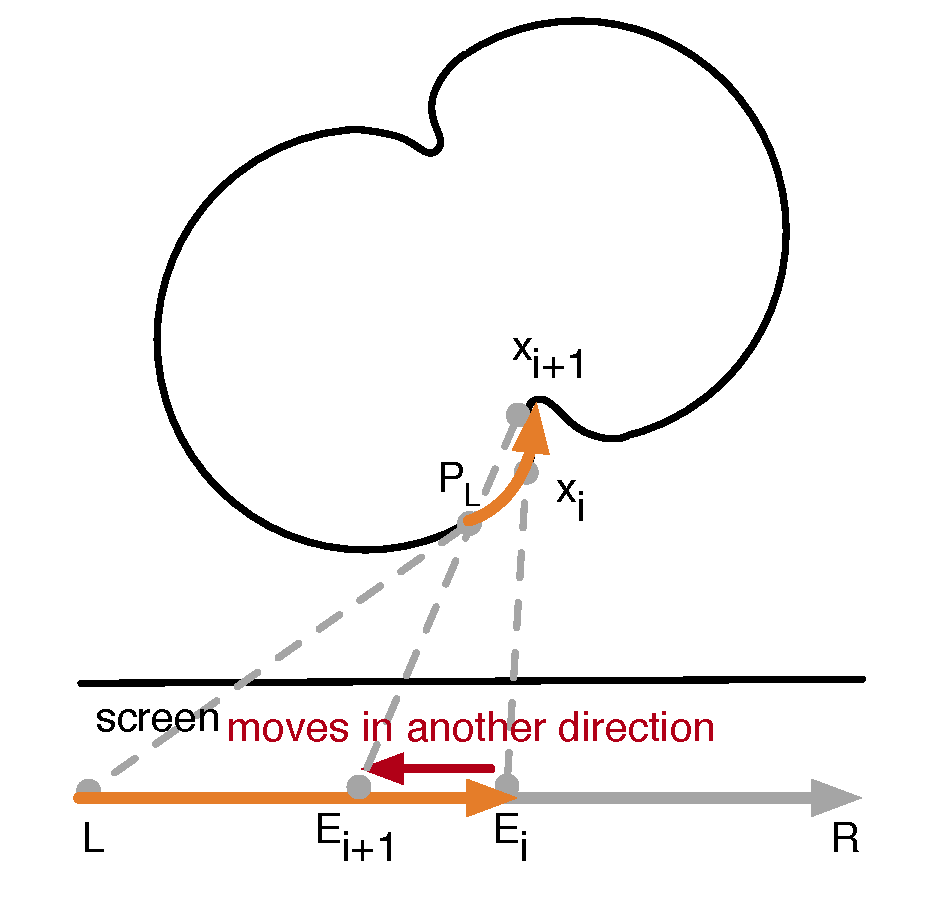
\includegraphics[width=.5\linewidth]{inverse_unslidable}\label{fig:inverse_not_slidable}}
    \caption{\epsl{}的推论。(a)表示$P_L$是\epslb{},(b)表示$P_L$不是\epslb{}} \label{fig:inverse_slidability}
\end{figure}

在这一章节中,本文将先对\citeauthor{kim2013stereoscopic}提出的\epsl{}\cite{kim2013stereoscopic}进行介绍,然后进一步阐述本文在此基础上进行的推导。

\section{\epsl{}}

以\con{}为例,如俯视图\autoref{fig:slidability}所示,\epsl{}的定义如下:假设$L$和$R$分别表示左眼和右眼对应的视点,$P_L$和$P_R$分别表示以$L$和$R$作为视点观察到的\con{}上的一个\conp{}。假设以$L$和$R$连线上的一个点$E$作为视点,当$E$从$L$向$R$移动,对应的轮廓点也应该从$P_L$向$P_R$移动,它在物体表面上移动的轨迹曲线${P_L}{P_R}$称为\ec{}\cite{geiger1995occlusions}。如果\ec{}上的轮廓点能够从$P_L$连续变化到$P_R$,那么$P_L$就是\epslb{}的(\autoref{fig:slidability}(a))。否则,如果\ec{}上的轮廓点能够从$P_L$连续变化到$P_R$,那么$P_L$不是\epslb{}的,不能和对应的轮廓点形成正确的立体视觉(\autoref{fig:slidability}(b)),因此该轮廓点应该在双目绘制的最终结果中被消去。
 
\citeauthor{kim2013stereoscopic}在他们的工作上提出了一种对$P_L$的\epsl{}进行检验的方法。具体来说,他们的方法首先在两眼对应的视点$L$和$R$之间枚举多个视点$E_0$、$E_1$……$E_n$,并按照顺序在这些视点上基于三维模型的几何绘制出轮廓线。当所有相邻视点得到的轮廓点,例如\autoref{fig:slidability}(a)中的$E_i$、$E_{i+1}$分别得到的$x_i$和$x_{i+1}$,都满足$x_{i+1}$在$x_i$的\ec{}方向上的一定区间范围内,那么就$P_L$就是\epslb{}的轮廓点。简而言之,就是为了确定当$E$从$L$向$R$移动时对应的轮廓点也相应地从$P_L$向$P_R$移动,所以通过从$L$向$R$按顺序采样多个视点并绘制出轮廓线的图像来进行验证。

需要特别指出的是,虽然以上定义和方法使用\con{}为例进行表述,但是以上定义和方法对于\scon{}也同样成立,例如$P_L$和$P_R$也可以分别表示以$L$和$R$作为视点观察到的\scon{}上的一个\sconp{}。在下文的讨论中,本文也会先以\con{}为例进行表述,在有需要特别说明的情况下,再对\scon{}的情况进行特别说明。

\section{\epsl{}的推论}

前人提出的\epsl{}的概念已在上一小节进行了细致的说明,它对于\conp{}和\sconp{}在双目绘制的情况下是否应该被消去给出了明确的数学判定条件,具有重要的指导意义。本文提出的方法则拓展了\epsl{}的概念并提出了一个推论:要判定\epsl{},可以通过检查$P_L$到$P_R$的轮廓点的对应视点的轨迹来完成,从而避免在$L$和$R$之间采样多个视点所需要的繁重的计算,使得设计更加高效的\stc{}的\con{}和\scon{}绘制算法成为可能。

本文提出的方法的出发点如\autoref{fig:inverse_slidability}所示。假设一个\conp{}$x$沿着$P_L$到$P_R$的\ec{}移动,如果$P_L$是\epslb{}的,那么$x$对应的视点$E$会单调地从$L$移动到$R$(\autoref{fig:inverse_slidability}(a))。如果$P_L$不是\epslb{}的,那么对应的视点$E$不会在到达$R$之前保持一直朝着$R$移动(\autoref{fig:inverse_slidability}(b))。简单来说,本文上述的判定过程在本质上和\citeauthor{kim2013stereoscopic}描述的\epsl{}的判定过程是一致是,只是本文是从\conp{}反推出视点的变化规律,并通过这个视点的变化规律来进行\epsl{}的判定,而不是像前人一样直接通过\conp{}的变化来进行\epsl{}的判定。

不难发现,以上提出的推论虽然以\con{}为例进行表述,但是对于\scon{}也完全适用。但是由于\con{}和\scon{}的数学定义不同,所以下面开始分别对\con{}和\scon{}用明确的数学语言给出有关\epsl{}的推论。

\subsection{\con{}}

基于上述的想法,对\epsl{}的判定可以转化为对对应视点的运动轨迹的单调性的判定。具体而言,假设有一个在\ec{}上移动的\conp{}$x$,对应的将$x$视为\conp{}的视点$E$可以用如下的公式计算:

\begin{equation}\label{eq:viewpoint2}
    {(E - P)}\cdot{N} = 0
\end{equation}

其中$P$和$N$分别表示\conp{}$x$的位置和法线方向,$E - P$表示视点$E$与$x$形成的视线方向。

又因为$E$位于$L$和$R$之间的连线上,所以它的位置可以用一个变量$t$进行以下的参数化:

\begin{equation}\label{eq:viewpoint1}
    E = (1-t)L+t R
\end{equation}

联立\autoref{eq:viewpoint2}和\autoref{eq:viewpoint1}可以得到:

\begin{equation}\label{eq:t1}
t = \frac{(P-L)\cdot{N}}{(R-L)\cdot{N}}
\end{equation}

\autoref{eq:t1}表示$t$是一个关于表面点$x$的函数。当$x$沿着\ec{}运动,$t(x)$就是轮廓点$x$的对应视点的轨迹函数。为了将\con{}和\scon{}对应的轨迹函数区分开来,本文使用$t_c(x)$来表示\conp{}的对应视点的轨迹函数,用$t_s(x)$来表示下文将要阐述的\sconp{}的对应的视点的轨迹函数,并用$t(x)$来对以上两种轨迹函数进行合称。

为了进一步讨论轨迹函数$t_c(x)$的单调性,本文将$t_c(x)$的导数形式计算如下:

\begin{equation}\label{eq:derivative}
    % \begin{split}
  t_c' = \frac{(P'\cdot{N}+(P-L)\cdot{N'})((R-L)\cdot{N})}{((R-L)\cdot{N})^2}-\frac{((R-L)\cdot{N'})((P-L)\cdot{N})}{((R-L)\cdot{N})^2}
    % \end{split}
\end{equation}

为了表达上的简洁,本文将\autoref{eq:derivative}中两边的$x$隐去。基于此公式,可以通过$t_c'(x)=0$找到极值点,从而判定轨迹函数的单调性在何时被破坏。该公式还可以作进一步的简化,使得计算起来更加简单。下面从$P(x)$和$N(x)$开始进一步的推导。

\begin{figure}[bth]
    \centering
    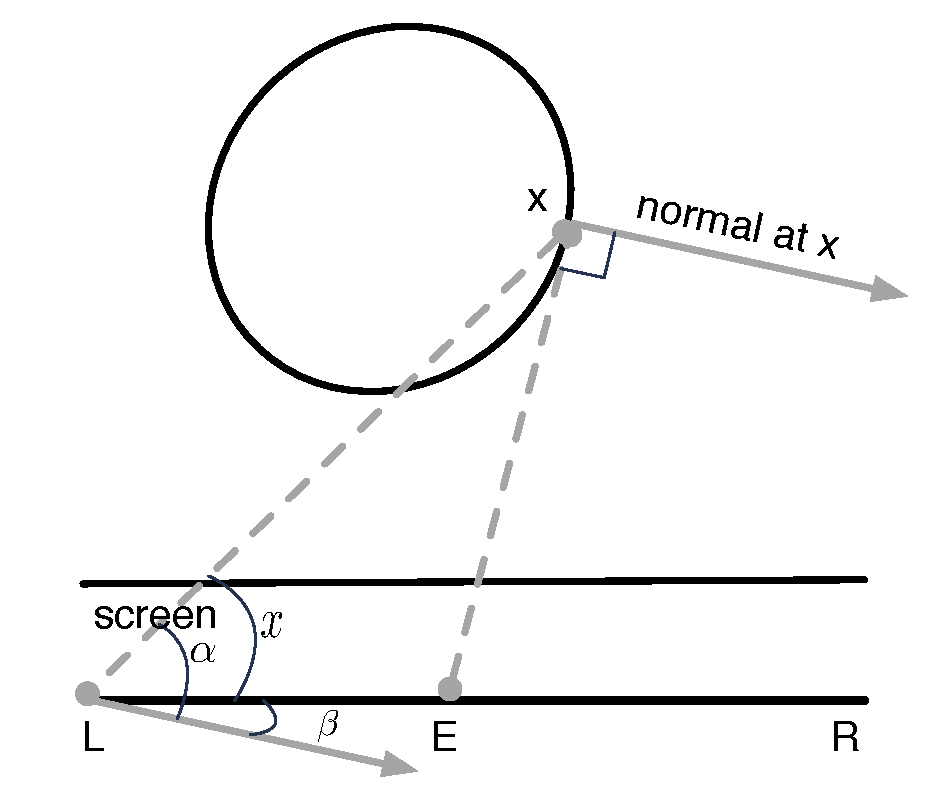
\includegraphics[width=0.6\linewidth]{deduction_t}
    \caption{\label{fig:deduction_t}
    $t$的导数的推导}
\end{figure}  

首先,$x$的位置$P(x)$的导数的方向正是该点的切线方向,换言之,$P'(x)$与法线方向垂直。因此有以下公式:

\begin{equation}\label{eq:perp}
    P'\cdot{N} = 0
\end{equation}

\begin{figure}[bth]
    \centering
    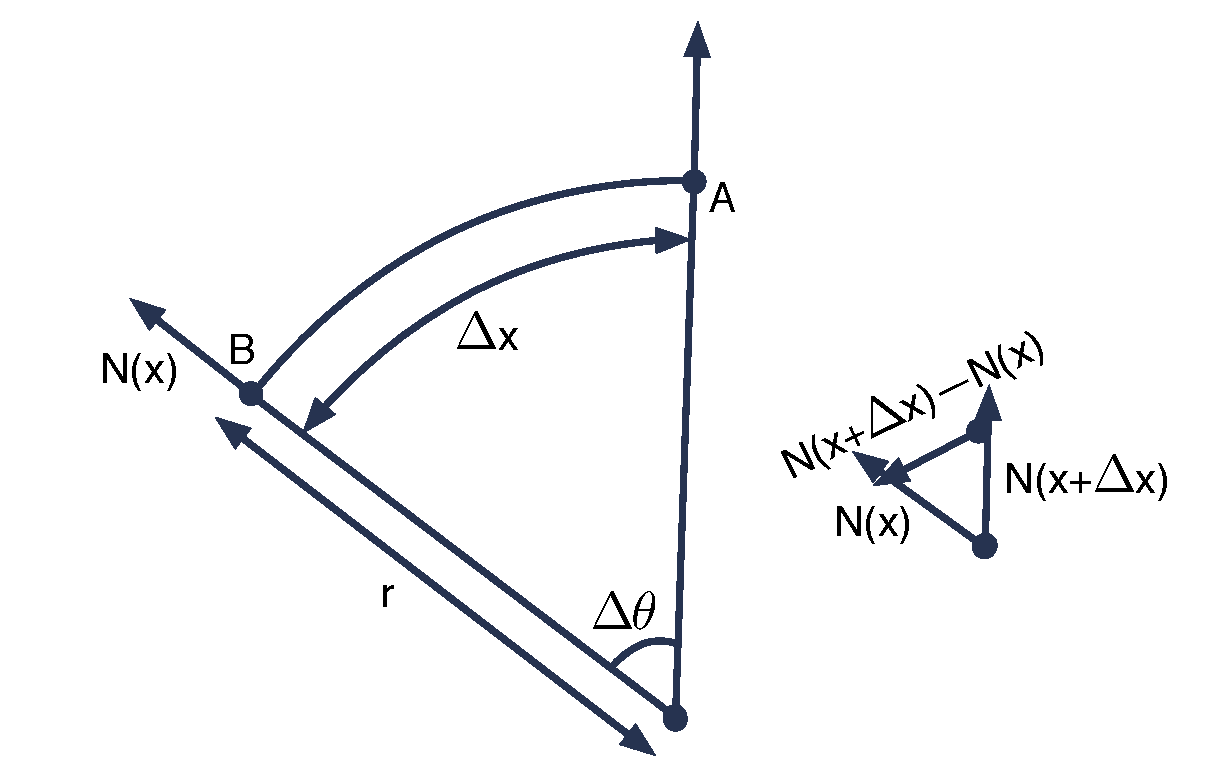
\includegraphics[width=0.6\linewidth]{deduction_n}
    \caption{\label{fig:deduction_n}
    曲线的法线导数的推导}
\end{figure}

再者,$x$的法线方向$N(x)$的导数可以进行以下的推导得出。首先,$N(x)$可以作为单位法线使用,原因如下:

\begin{equation}
    t_c = \frac{(P-L)\cdot{N}}{(R-L)\cdot{N}} = \frac{(P-L)\cdot{\frac{N}{|N|}}}{(R-L)\cdot{\frac{N}{|N|}}}
\end{equation}

接着,正如\autoref{fig:deduction_n}所示,当$P(x+\Delta x)$从$A$移动到$B$,$N(x)$,$N(x+\Delta x)$和$N(x+\Delta x)$ - $N(x)$组成来一个等腰三角形,因为$N(x)$和$N(x+\Delta x)$都是单位法线。因此可以得出:

\begin{equation}
    |N(x+\Delta x) - N(x)| = \Delta\theta \cdot 1 = \Delta\theta = |N'(x)\Delta x|
\end{equation}

又由于$\Delta x \to 0$,所以

\begin{equation}\label{eq:curvature}
    |N'(x)| = \lim_{x \to 0}\frac{\Delta\theta}{\Delta x} = \lim_{x \to 0}\frac{\Delta\theta}{r\Delta\theta} = \frac{1}{r} = C(x)
\end{equation}

其中$C(x)$表示\ec{}上一点$x$的曲率。另外,当$\Delta x \to 0$,$|N(x+\Delta x) - N(x)|$的方向趋近于与法线$N(x)$的方向垂直,因此可以得到$N'(x) \perp N(x)$。假设 $\alpha$表示$P(x)-L$和$N(x)$之间的夹角,$\beta$表示$R-L$和$N(x)$之间的夹角,可以进行如下的转化:

\begin{equation}\label{eq:alpha}
(P-L)\cdot{N'} = |P-L|{|N'|}\cos{(\alpha+\frac{\Pi}{2})} = |P-L|{|N'|}\sin\alpha
\end{equation}

\begin{equation}\label{eq:beta}
(R-L)\cdot{N'} = |R-L|{|N'|}\cos{(\beta+\frac{\Pi}{2})} = |R-L|{|N'|}\sin\beta
\end{equation}

结合\autoref{eq:derivative},\autoref{eq:perp},\autoref{eq:curvature},\autoref{eq:alpha}和\ref{eq:beta},可以得到:

\begin{equation}\label{eq:final}
\begin{split}
t_c' & = \frac{C|P-L||N|\sin\alpha|R-L||N|\cos\beta-C|R-L||N|\sin\beta|P-L||N|\cos\alpha}{((R-L)\cdot{N})^2} \\
& = \frac{C|P-L||R-L||N|^2(\sin\alpha\cos\beta-\sin\beta\cos\alpha)}{((R-L)\cdot{N})^2} \\
& = \frac{C|P-L||R-L||N|^2\sin(\alpha-\beta)}{((R-L)\cdot{N})^2} \\
& = \frac{C|P-L||R-L||N|^2\sin(\gamma)}{((R-L)\cdot{N})^2}
\end{split}
\end{equation}

正如\autoref{fig:deduction_t}所示,$\gamma$是$P(x)-L$和$R-L$之间的夹角。由于$x$ 位于$L$与$R$连线的正前方,$sin\gamma$的值恒大于0。因此,$t_c'(x)$的符号只与$C(x)$有关。

需要明确指出的是,由于三维模型的不连续性,$t_c'(x)=0$在模型上出现的位置并不是连续的。因此,本文将通过$t_c'(x-)t_c'(x+) < 0$而不是$t_c'(x)=0$来找出极值点。

在本文设计的方法中,会将\ec{}上的\conp{}投影到左眼和右眼对应的图像,再沿着极线(epipolar line)而不是物体空间中的\ec{}(epipolar curve)进行搜索。这样一来,即可计算出极值点并存储到图像空间,从而在图像空间实现\epsl{}的判定。

\subsection{\scon{}}
\label{sec:suggestive_contour_math}
通过检测对应视点的轨迹的想法同样可以应用到\scon{}上。\scon{}的定义如下:

\begin{align}
  \kappa_r &= 0 \label{eq:Kr} \\
  D_w\kappa_r &> 0 \label{eq:DwKr} 
\end{align}

其中$\kappa_r$表示表面上一点的径向曲率,$D_w\kappa_r$表示$\kappa_r$的方向导数。更确切地说,$\kappa_r$是视线方向$V$在切平面上的投影$W$的方向上的法向曲率。法向曲率以及方向导数的概念已经在\autoref{sec:diff_geo}中进行说明,在此不再赘述。$\kappa_r$可以用以下形式表示为关于主曲率和$W$的函数:

\begin{equation}\label{eq:normal curvature}
    \kappa_r = \kappa_1cos^2\phi+\kappa_2sin^2\phi
\end{equation}

其中$\kappa_1$和$\kappa_2$是两个主曲率,$\phi$是$W$的方向与$\kappa_1$对应的主曲率方向(principal curvature direction)。为了找到\scon{}与视点之间的对应关系,将$\kappa_r = 0$代入\autoref{eq:normal curvature},并结合$cos^2\phi + sin^2\phi = 1$,可以得到:

\begin{align}
    cos^2\phi &= \frac{\kappa_2}{\kappa_2-\kappa_1} \label{eq:cos}\\
    sin^2\phi &= \frac{-\kappa_1}{\kappa_2-\kappa_1} \label{eq:sin}
\end{align}

从\autoref{eq:cos}和\autoref{eq:sin}中可以分别获知满足$\kappa_r = 0$的$W$与主方向$D_1$形成的夹角的余弦值和正弦值。于是,假设$\kappa_1$和$\kappa_2$满足$\kappa_1\kappa_2 \leq 0$,可以按照以下形式计算出满足$\kappa_r = 0$的$W$:

\begin{align}
    W &= cos{\phi}D_1+sin{\phi}D_2 \\
    &= \pm\sqrt{\frac{\kappa_2}{\kappa_2-\kappa_1}}D_1\pm\sqrt{\frac{-\kappa_1}{\kappa_2-\kappa_1}}D_2 \label{eq:w}
\end{align}

其中$D_1$和$D_2$是分别是对应的主曲率的方向。尽管\autoref{eq:w}中$\kappa_r = 0$的解有四个,但是由于视点$E$观察到的三维模型上的一点$x$必然位于$E$的前方,所以$\kappa_r = 0$的四个解中只有其中两个可以是$L$和$R$之间一个视点$E$的视线方向的投影(另外的两个解所代表的方向与这两个解代表的方向完全相反)。

\begin{figure}[tbp]
    \centering
    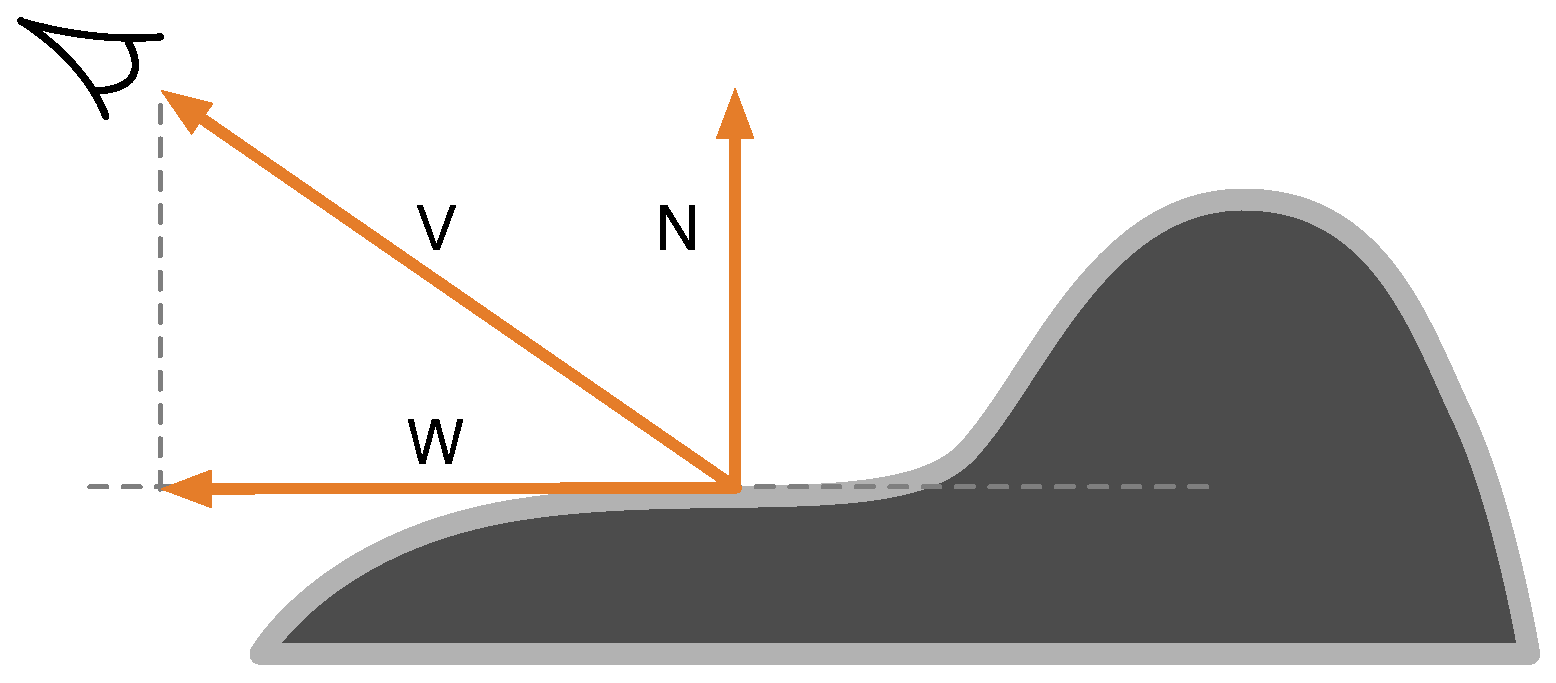
\includegraphics[width=0.9\linewidth]{suggestive_contour_definition}
    \caption{\label{fig:suggestive_contour_definition2}
    \scon{}的定义。其中$N$表示表面法线,$V$表示视线方向,$W$表示$V$在切平面上的投影。}
\end{figure}

至此,本文得出了将表面点$x$视为\sconp{}的$W$的表达式,但是还未建立将表面点$x$视为\sconp{}的视点$E$的与$x$上的几何特征所存在的直接关系。为了建立这一关系,需要回顾\autoref{fig:suggestive_contour_definition2}中展示的\scon{}的定义。由于$W$是$V$在切平面上的投影,所以在确定$W$后,$V$必须要位于$W$和$x$上的法线$N$形成的面内。换言之,假设将$W$和$x$上的法线$N$的叉积记为$M$:

\begin{equation}\label{eq:suggestive viewpoint}
    M = W \times N
\end{equation}

那么,视点$E$观察点$x$所形成的视线方向必定垂直于$M$。所以,将某个表面点视为\sconp{}的视点$E$必须满足:

\begin{equation}\label{eq:suggestive viewpoint}
    {(E - P)}\cdot{M} = 0
\end{equation}

不难看出,由于\autoref{eq:suggestive viewpoint}的形式和\autoref{eq:t1}一致,同样地,可以将视点$E$用一个参数$t$参数化成\autoref{eq:viewpoint1}的形式并推导出$t$的表达式:

\begin{equation}\label{eq:suggestive trajectory}
    t = \frac{(P-L)\cdot{M}}{(R-L)\cdot{M}}
\end{equation}

该公式表示了\scon{}的对应视点的轨迹函数,也就是$t_s(x)$。同样地,基于$t_s(x)$可以计算出极值点从而对\scon{}的\epsl{}进行判定。然而,与\con{}不同的是,对于每个\sconp{}会有两个对应的视点将其视为\sconp{},所以$t_s(x)$是一个多值函数(multivalued function)。关于\scon{}的极值点的计算细节将在\ref{sec:suggestive_contour_algorithm}中进一步阐述。

另外,关于$t_s(x)$的推导是建立在$\kappa_1\kappa_2 \leq 0$的假设的前提下的,如果$x$上的两个主曲率不满足$\kappa_1\kappa_2 \leq 0$,那么就不存在使$\kappa_r = 0$成立的方向$W$,也不存在对应的视点将$x$视为\sconp{}。

与$\kappa_1\kappa_2 \leq 0$类似,还有其他条件会使得不存在对应的视点将$x$视为\sconp{}。在上述的讨论中,\scon{}的另一个决定条件$D_w\kappa_r>0$还没有考虑在内。同样地,如果$x$上的径向曲率$\kappa_r$的方向导数不满足$D_w\kappa_r>0$,那么即使$x$能够找到满足$\kappa_r = 0$的对应视点,该点也不会被视为\sconp{}。

再者,在实际运用中,还会用以下的条件来进一步限制\scon{}的出现范围:

\begin{equation}\label{eq:cosNdotV}
  cos^{-1}(N\cdot{V}) > \theta_c 
\end{equation}

其中$\theta_c$是一个用户设定的常量。由于直接通过定义检测得到的\scon{}并不稳定,在画面上来看会随着视点和三维模型相对位置的变化而剧烈变化,造成画面闪烁、线条看起来不连续的现象。因此,在实际运用中会通过\autoref{eq:cosNdotV}中的条件来进一步对按照定义检测出的\scon{}进行筛选,去掉这些不稳定的部分的\sconp{}。

综上所述,对于那些不符合上述三个条件的表面点,不存在对应的视点将其视为\sconp{}。换言之,$t_s(x)$的区间端点有三种:

\begin{enumerate}
\item $\kappa_1\kappa_2 = 0$
\item $D_w\kappa_r = 0$
\item $cos^{-1}(N\cdot{V}) = \theta_c$
\end{enumerate}

满足上述三个条件之一的点都是$t_s(x)$的区间端点。除了极值点以外,这些区间端点也会破坏对应视点的轨迹的单调性。因此,对于\scon{}来说,要实现\epsl{}的判定,除了计算出极值点外,还需要计算出这些区间端点并将它们存储到\ppll{}。
% 在后续的图像空间搜索来判定\epsl{}时,这些区间端点的作用和极值点相同,都是判定\sconp{}不是\stc{}并停止搜索的依据。
\chapter{\stc{}\con{}和\scon{}绘制算法}

基于上一章的推导,可知\epsl{}可以通过检查轨迹函数$t(x)$的极值点来在图像空间中完成判定。因此,本文设计了一个算法来实现\stc{}\con{}和\scon{}绘制,并实时完成\epsl{{}的判定。在这一章中,本文将针对\con{}对整个算法流程进行总结,并对流程中每个阶段的细节进行具体的说明,再讲述如何将这套算法拓展至\scon{}上,以及如何实现进一步的线条风格化。

\begin{figure}[tbh]
    \centering
    \makebox[\textwidth][c]{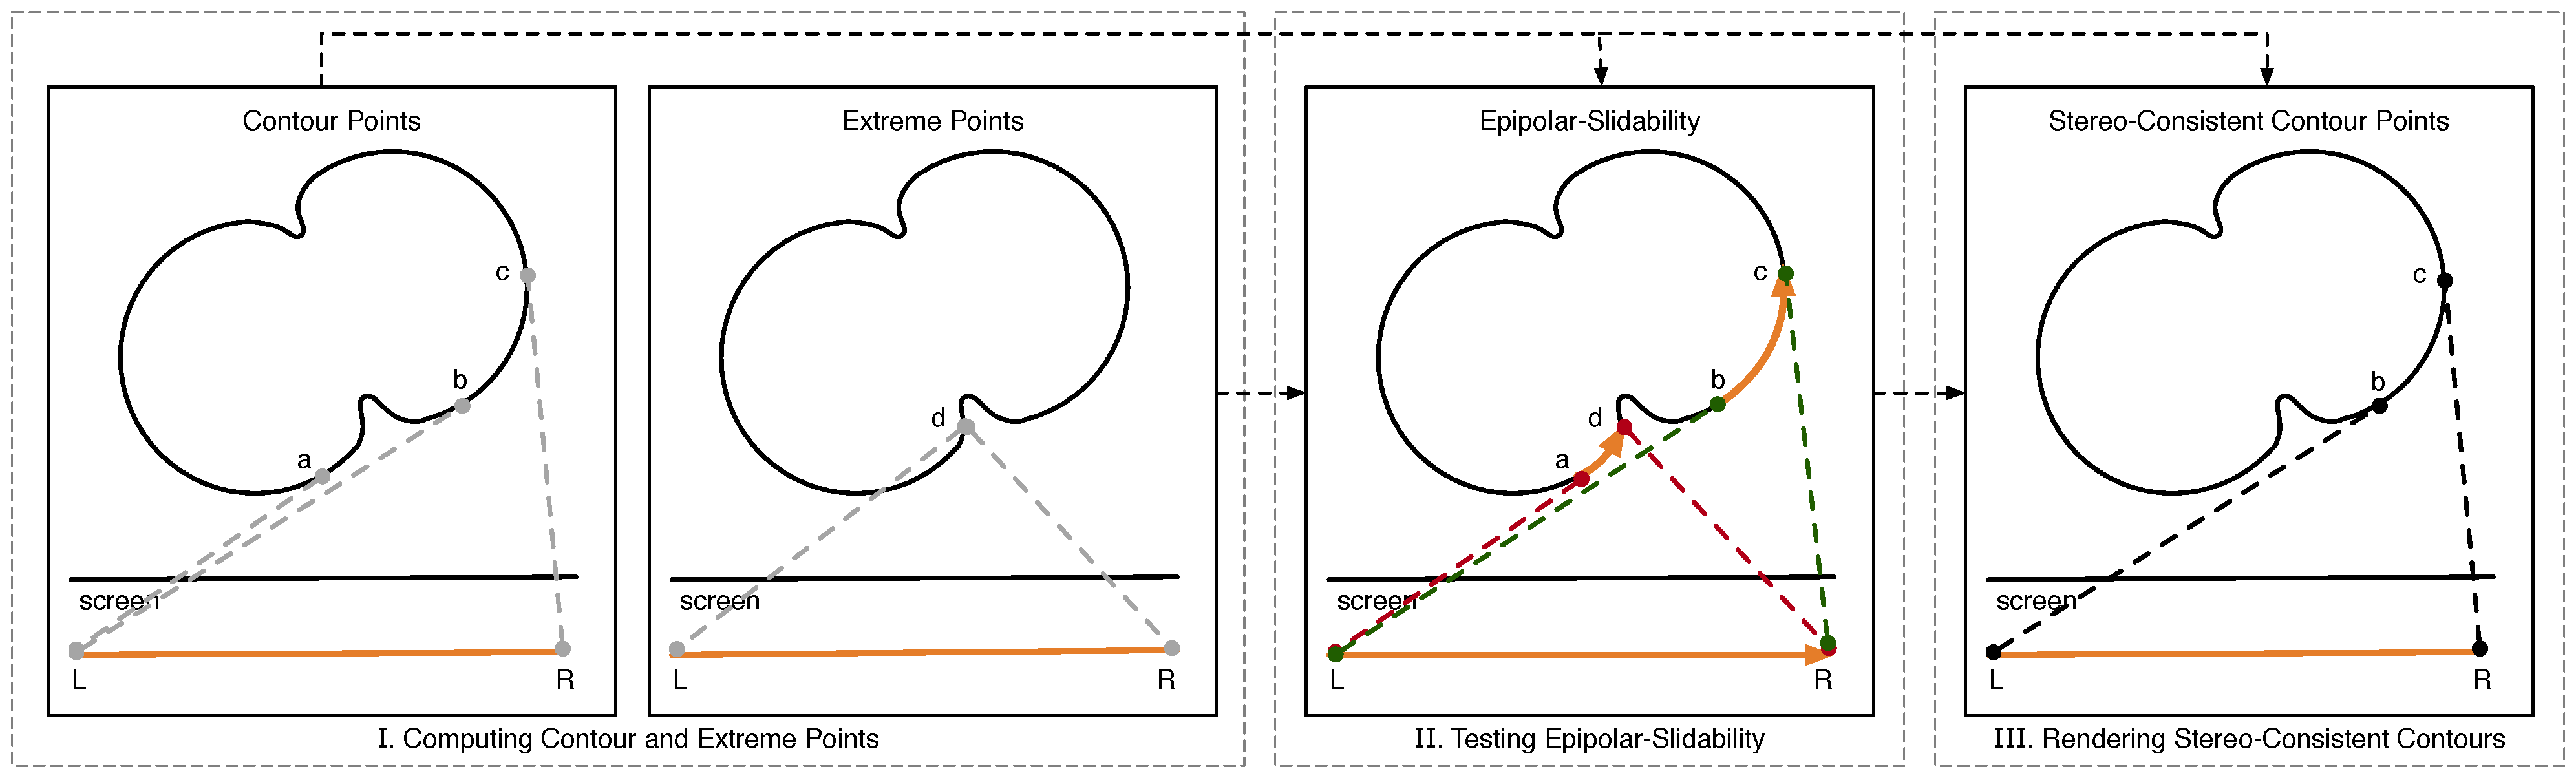
\includegraphics[width=1.2\linewidth]{overview2}}
    \caption{\label{fig:overview2}
    算法流程说明。为了描述上的简洁,该说明只展示了从$L$到$R$计算\stc{}\con{}的过程。首先,\conp{}$a$、$b$、$c$和极值点$d$被计算出来。其次,本文设计的算法在图像空间中对$a$和$b$的\epsl{}进行判定,其中$a$由于遇到了$d$所以判定为不是\stc{},而$b$由于找到了对应的来自右眼的\conp{}$c$所以判定为\stc{}。最后,将\stc{}的\conp{}$b$和$c$绘制到最终展示的两眼对应图像中。
    }
\end{figure}

\autoref{fig:overview2}对本文提出的算法流程进行了说明,其中主要包含以下三个步骤:
\begin{enumerate}[label=\textbf{\Roman*.},leftmargin=*,align=left,labelwidth=\parindent,labelsep=0pt]
    \item \textbf{计算轮廓点和极值点:} 首先,在每一帧的开始阶段,绘制基础的\conp{}和极值点并将它们存储到\ppll{}中。
    \item \textbf{\epsl{}的判定:} 接着,采用一个图像空间的搜索算法,完成对上一步得到的\con{}的\epsl{}的判定。
    \item \textbf{绘制\stc{}\con{}:} 最后,将所有的\epslb{}的\con{}绘制到两眼对应的图像中。
\end{enumerate}

\begin{figure}[tbh]
    \centering
    \makebox[\textwidth][c]{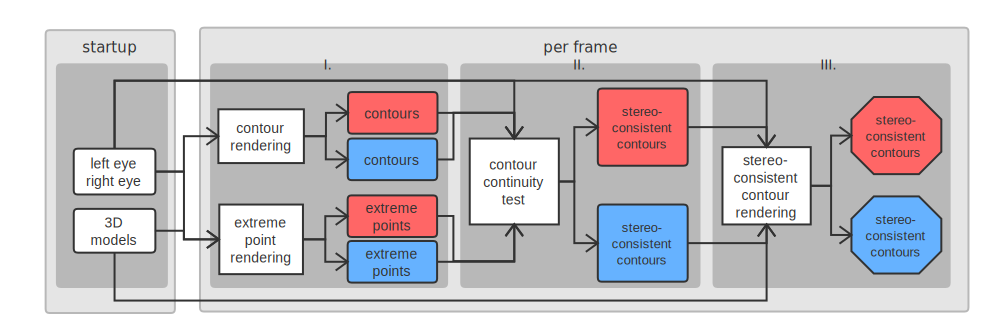
\includegraphics[width=1.2\linewidth]{overview}}
    \caption{\label{fig:overview}
    系统总览。蓝色/红色的正方形表示左眼/右眼的某种实例。在初始化阶段,首先载入三维模型并对对应于两眼的摄像机进行设置。在后续的每一帧中,轮廓点和极值点先是被绘制并存储到\ppll{}上,然后以这些\ppll{}作为输入进行\epsl{}的判定,最后,基于上一步得到的\epsl{}绘制出\stc{}轮廓线。}
\end{figure}

在上述算法的基础上,本文设计了一个如\autoref{fig:overview}所示实时绘制系统。下面将分别对各个阶段进行进一步的说明。

\section{计算\conp{}和极值点}

在第一个阶段,本文设计的算法先对模型进行光栅化并计算出\conp{}和极值点。如果将\scon{}也考虑在内,那么\scon{}和对应的极值点和区间端点也需要在这个阶段完成计算。下面的两个小节将分别针对\con{}和\scon{}的计算方法进行进一步的说明。需要特别指出的是,关于\con{}和\scon{}的基本绘制已在\autoref{sec:basic}中提及,因此在下文中不再赘述。

\subsection{\con{}}

为了计算极值点,也就是满足$t_c'(x-)t_c'(x+) < 0$的点,本文在前一章节中的推导中得出$t_c'(x)$的表达式的正负只与$C(x)$有关。因此,本文设计的方法通过$C(x-)C(x+) < 0$而不是$t_c'(x-)t_c'(x+) < 0$来计算出\con{}对应的极值点,这样一来计算更加简单。上述的$C(x)$表示$x$处的曲率,可以在三维模型的每个三角形上以类似于通过$N\cdot{V} = 0$来找到\conp{}的方式计算出来。

然而,基于下面的原因,本文采取一种更为精确的方法来计算出这些极值点。在三维模型被光栅化之后,每个片段上的法线值是基于重心坐标对顶点法线进行插值得到的。因此,如果将一条对极曲线投影到一个三角形上,沿着投影线的法线变化必然是线性连续的,说明$C(x)$在三角形内是一个常量。

轮廓点与极值点之间可能会存在重叠,例如多个轮廓点和极值点都处在图像空间的同一个像素上。因此,本文使用了\ppll{}来存储同一个像素上的轮廓点和极值点。考虑到轮廓点和极值点只占图像空间中的一小部分,使用\ppll{}带来的内存占用是完全可以接受的。

\begin{figure}[tbh]
    \centering
    \subfloat[左眼]{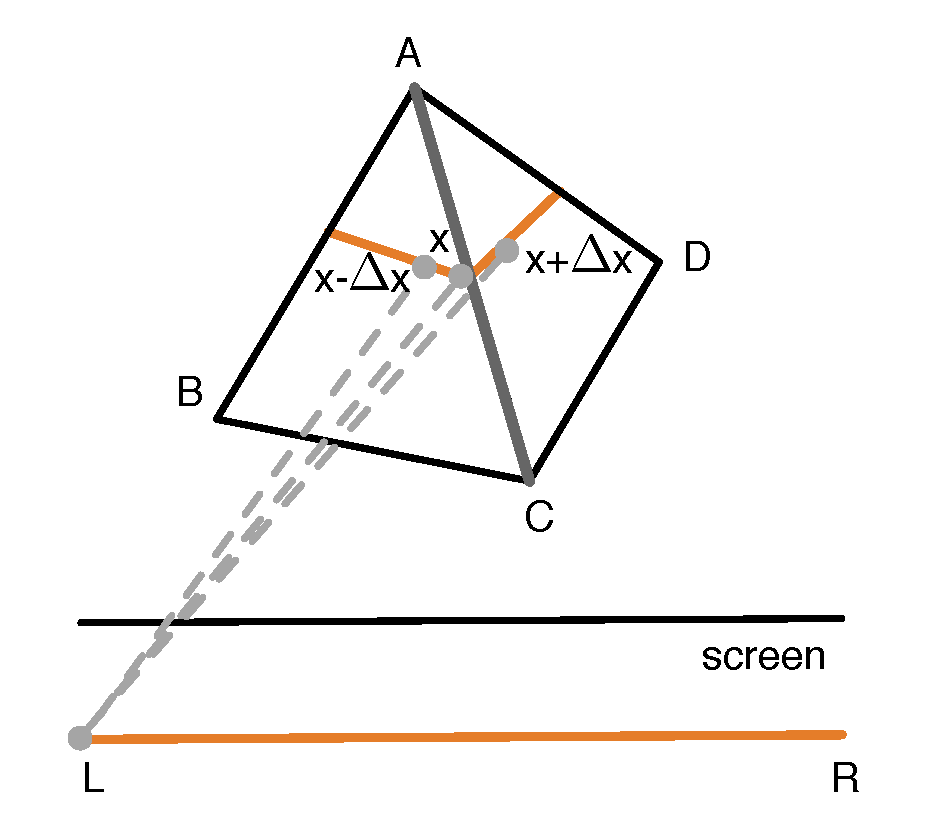
\includegraphics[width=.5\linewidth]{inflection_line_left}}
    \hfil
    \subfloat[右眼]{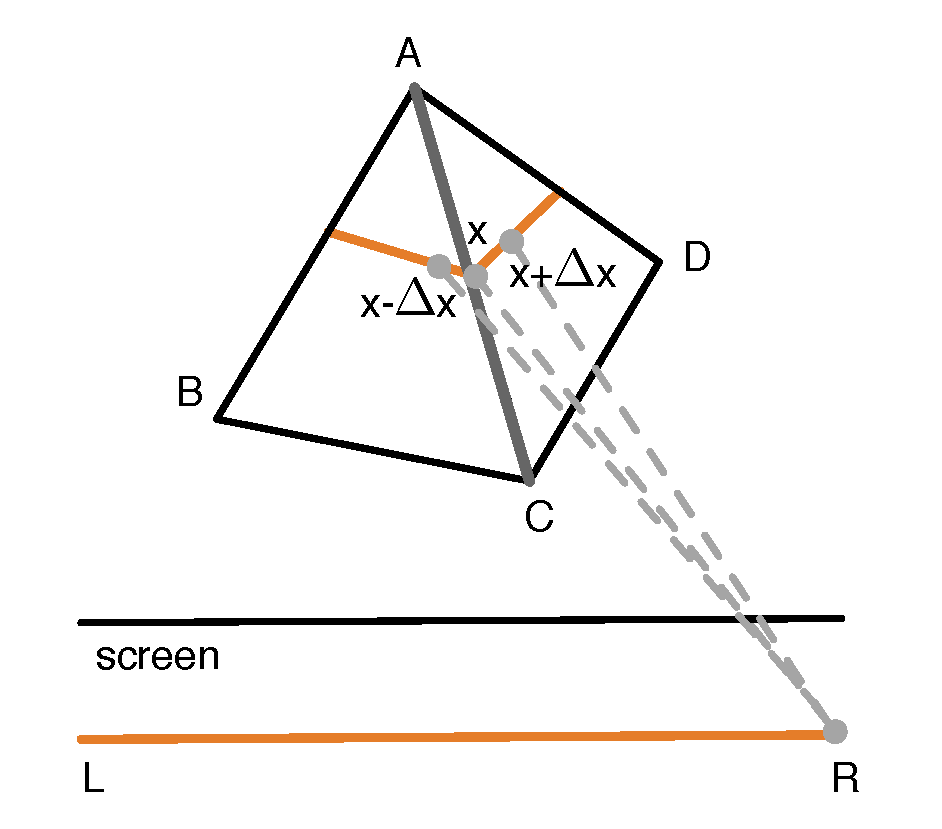
\includegraphics[width=.5\linewidth]{inflection_line_right}}
    \caption{极值点的计算。$\triangle ABC$和$\triangle ACD$是两个相邻的三角形。本文设计的方法对位于边$AC$上的每个片段进行极值点的判定。(a) 在左眼的图像空间计算极值点。 (b) 在右眼的图像空间计算极值点。} \label{fig:extreme points}
\end{figure}

\subsection{\scon{}}

\begin{figure}[tbh]
    \centering
    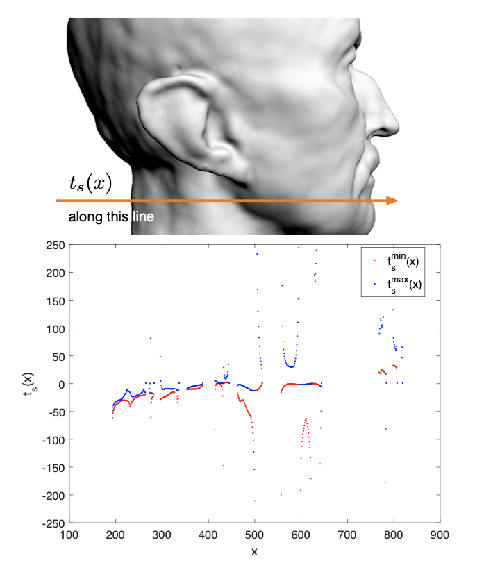
\includegraphics[width=\linewidth]{ts_example.eps}
    \caption{\label{fig:continuity_example}
    $t_s(x)$的一个例子。该图表示沿着图像中某一行的$t_s(x)$的值的分布。蓝色/红色的点分别表示$t_s^{max}(x)$/$t_s^{min}(x)$的值。}
\end{figure}

\begin{figure}[tbh]
    \centering
    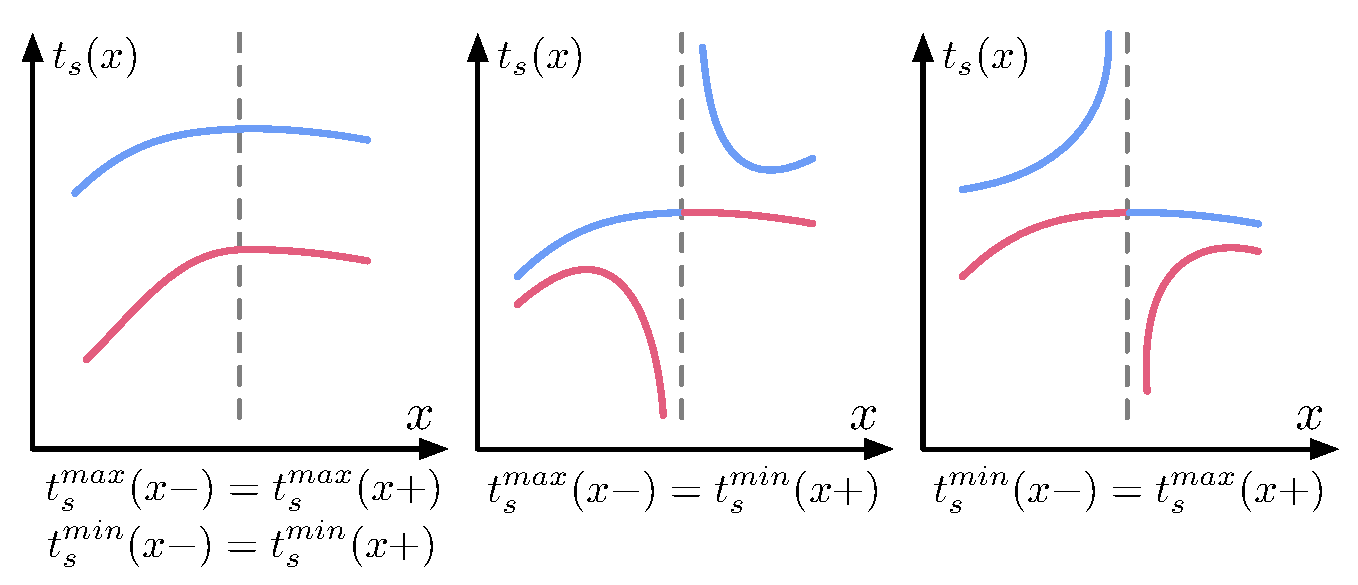
\includegraphics[width=.95\linewidth]{continuity}
    \caption{在虚线所指位置上,$t_s(x)$的连续性的三种不同情况。}
    \label{fig:ts_continuity}
\end{figure}

\label{sec:suggestive_contour_algorithm}

正如本文在\ref{sec:suggestive_contour_math}中讨论的那样,对于\scon{}的\epsl{}的判定,除了需要计算轨迹函数的极值点外还需要计算出区间端点。同样地,本文采用了与绘制\con{}的方法相似的方法来计算出区间端点,也就是满足$\kappa_1\kappa_2 = 0$,或者$D_w\kappa_r = 0$,又或者$cos^{-1}(N\cdot{V}) = \theta_c$的那些点。

计算$t_s(x)$的极值点比计算$t_c(x)$的极值点要更加困难。对于\con{},基于上文\autoref{eq:curvature}所述的推导,只需要在三角形的边上进行计算即可。但是对于\scon{}而言,不存在同样的性质,所以不仅需要在边上也需要在三角形内进行计算。再者,与通过$C(x)$来找到间接地找到极值点不同,只能通过对比多个连续的$t_s(x)$的值来直接地找到$t_s(x)$的极值点。

另外,考虑到$t_s(x)$是一个对于每个点有两个取值的多值函数,必须要在通过对比$t_s(x)$的连续几个值来决定极值点前确定$t_s(x)$的多个值的连续性。为了将$t_s(x)$的两个值区分开来,本文使用$t_s^{min}(x)$和$t_s^{max}(x)$来分别表示它们中的最小值和最大值。\autoref{fig:continuity_example}展示了$t_s(x)$的一个例子。一般而言,$t_s^{min}(x)$和$t_s^{max}(x)$在大部分点上是分别连续的,但是在某些点上也会相互连续。\autoref{fig:ts_continuity}总结了$t_s(x)$的三种不同的连续情况。具体来说,本文设计的方法首先
在片段着色器中计算出三个连续的$t_s^{min}(x)$和$t_s^{max}(x)$的值,并按照这些值的关系对应到\autoref{fig:ts_continuity}中的其中一种情况。然后,对比对应的连续三个值来确定此处是否为极值点。需要特别指出的是,在\autoref{fig:ts_continuity}的情况(a)中可能会在同一个点上同时存在$t_s^{min}(x)$和$t_s^{max}(x)$的局部最小值。无论是哪一种情况,只要$t_s^{min}(x)$或者$t_s^{max}(x)$的局部极值出现,就应该将其存储为极值点。

\section{\epsl{}的判定}

\begin{figure}[tbh]
    \centering
    \subfloat[不需要重投影的搜索]{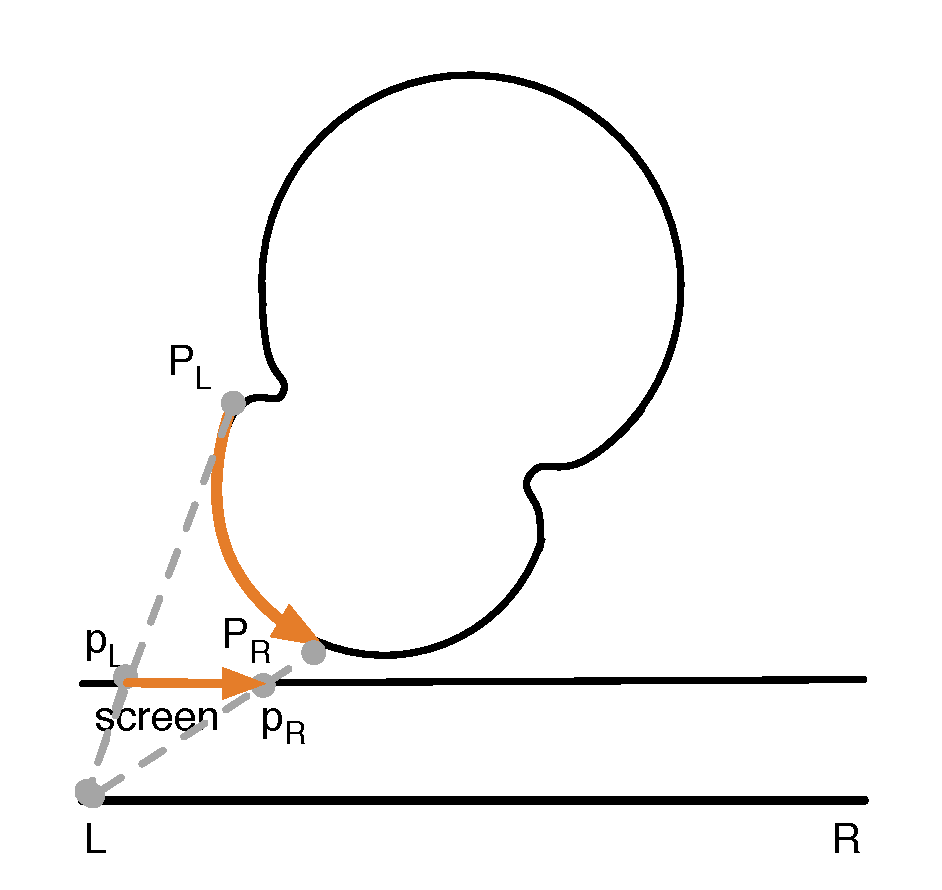
\includegraphics[width=.5\linewidth]{search_leftside_2}}
    \hfil
    \subfloat[需要重投影的搜索]{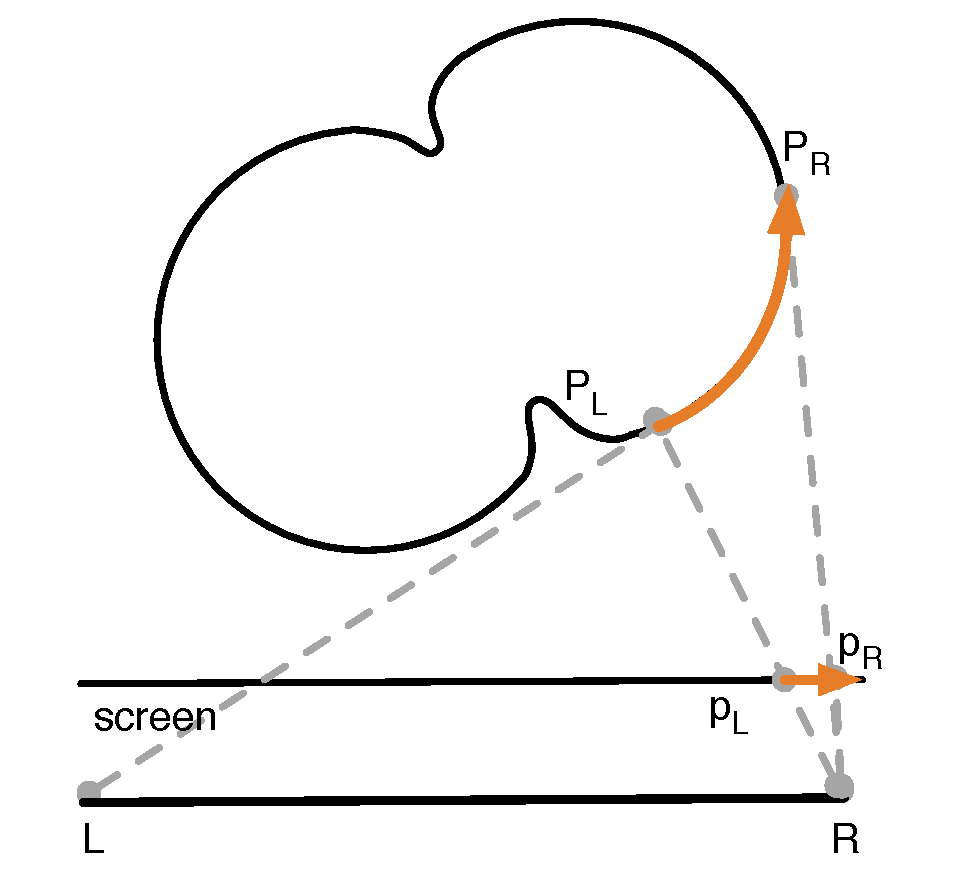
\includegraphics[width=.5\linewidth]{search_rightside}}
    \caption{遇到对应轮廓点的搜索过程。$p_L$和$p_R$分别表示$P_L$和$P_R$的投影。}\label{fig:succeed in image space search}
\end{figure}

\begin{figure}[tbh]
    \centering
    \subfloat[需要重投影的搜索]{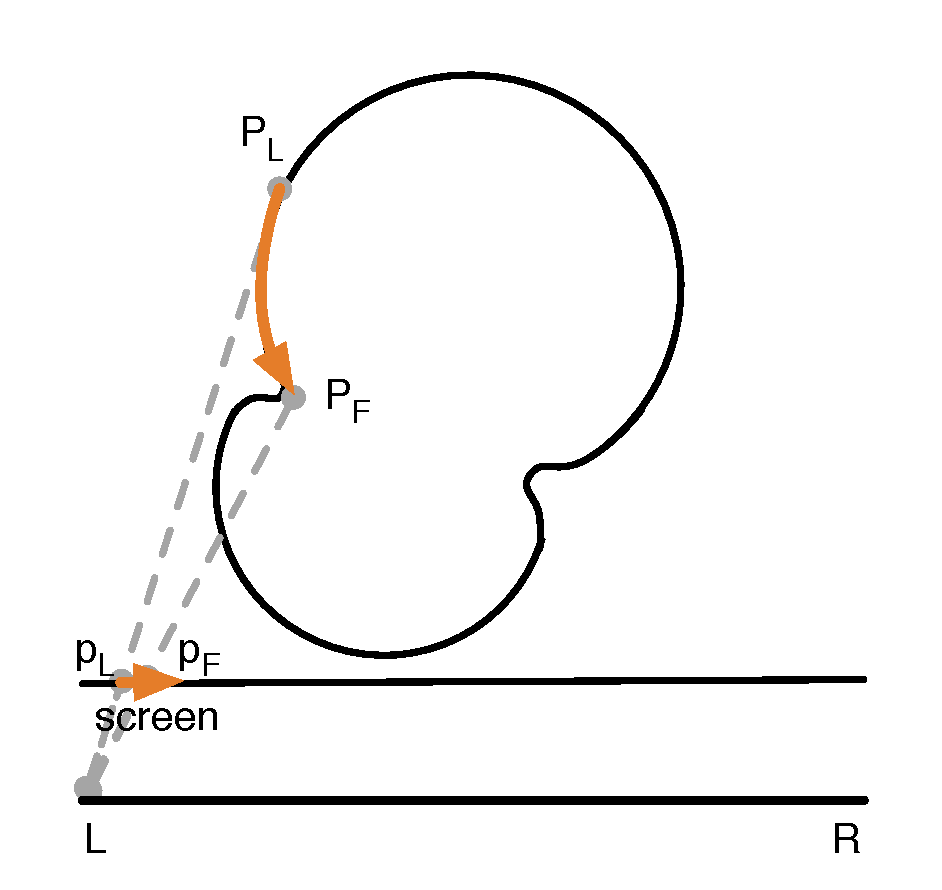
\includegraphics[width=.5\linewidth]{search_leftside_fail_2}}
    \hfil
    \subfloat[需要重投影的搜索]{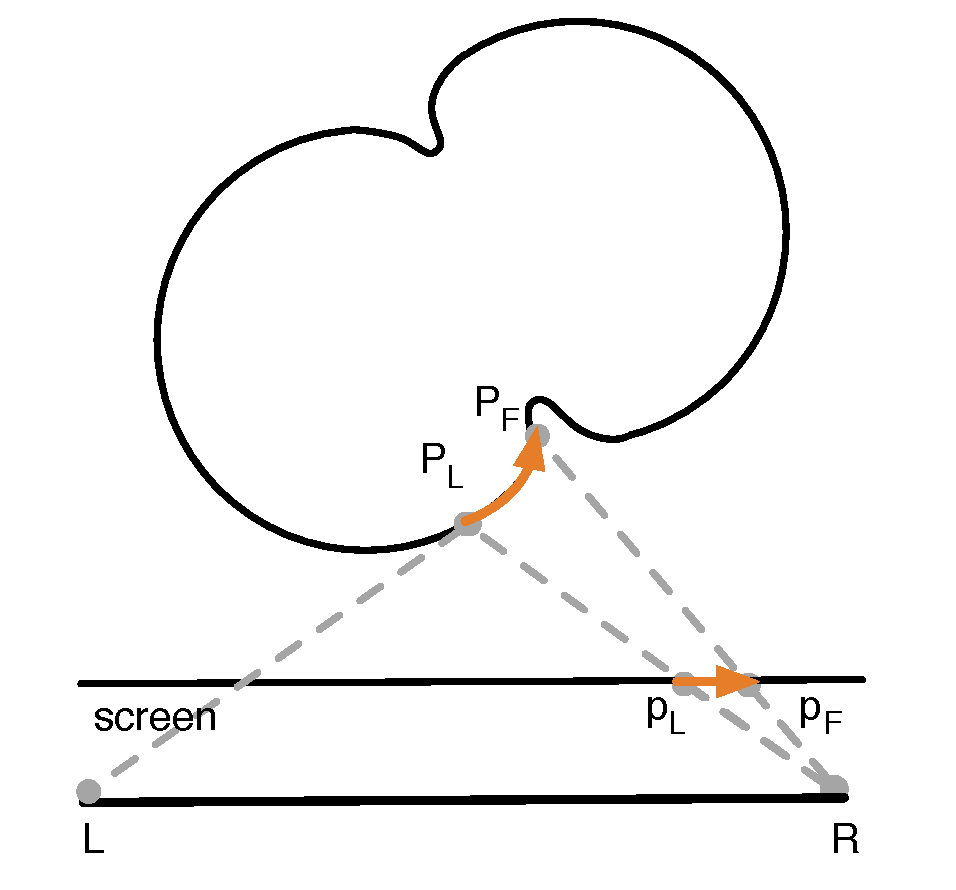
\includegraphics[width=.5\linewidth]{search_rightside_fail}}
    \caption{在极值点处停止的搜索过程。$P_F$是一个极值点。$p_L$和$p_F$分别表示$P_L$和$P_F$的投影。} \label{fig:fail in image space search}
\end{figure}

\begin{figure}[tbh]
    \centering
    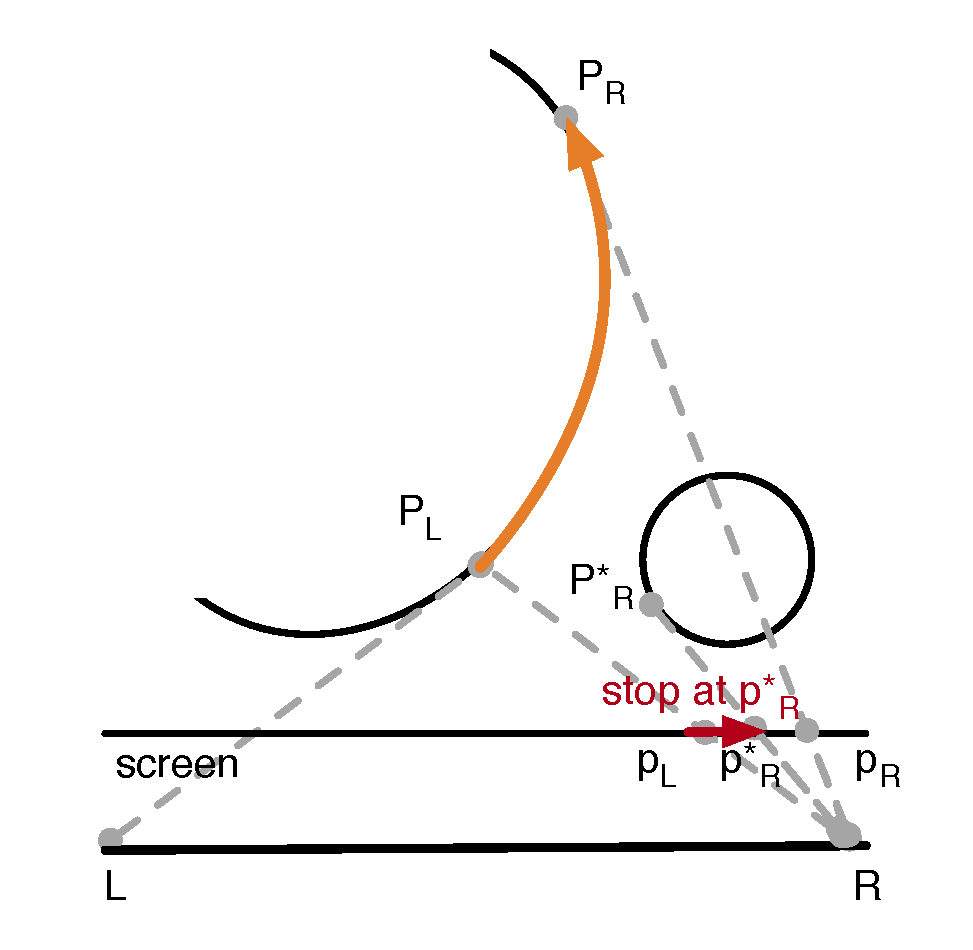
\includegraphics[width=0.6\linewidth]{search_occlude}
    \caption{\label{fig:occlude}
    由于遮挡导致的错误匹配。本文设计的方法通过物体的索引来排除这种情况。}
\end{figure}

本文使用两个全屏后处理来分别实现左眼和右眼两个图像上的\epsl{}的判定。本文设计的用于\epsl{}判定的搜索算法主要有以下三步:

\begin{enumerate}
    \item 在有需要的情况下,将\conp{}从当前视点的图像空间重投影到另一视点的图像空间。
    \item 根据\conp{}所观察的视点是左眼还是右眼,判定搜索方向(从左往右或者从右往左)。
    \item 在图像空间中逐个像素进行搜索。对于每个像素,遍历并检查存储在\ppll{}上的每个点。当遇到存有另一视点下的对应\conp{}的像素或者遇到极值点时,搜索停止。
\end{enumerate}

\autoref{fig:succeed in image space search}展示了遇到对应\conp{}的两个搜索过程,其中一个在起始位置做了重投影,另外一个没有在起始位置做重投影。而\autoref{fig:fail in image space search}展示了遇到在极值点处停止的搜索过程。下面以从$L$到$R$的搜索过程为例来阐述具体每个步骤的细节,从$R$到$L$的搜索过程是相似的。

{\textbf{重投影:} 如果\conp{}的表面法线指向视线方向的右边,则将\conp{}从当前视点的图像空间重投影到另一视点的图像空间。否则,不需要做重投影。法线指向视线方向的右边还是左边可以用明确的数学语言进行表述。如果视线方向和表面法线方向的叉积,也就是$cross(N, V)$,指向对极平面的上方,则表示\conp{}的法线方向指向视线方向的左边,反之亦然。

\textbf{搜索方向:} 搜索方向决定于将该点视为\conp{}的是左眼还是右眼。如果\conp{}是从左眼观察得到的,那么从左往右搜索。否则,从右往左搜索。

\textbf{错误匹配的排除:} 当对极曲线被其他物体所遮挡时,可能会产生错误的匹配结果。\autoref{fig:occlude}展示了这样的一个例子,其中${P^*}_R$是一个位于另外一个物体上的\conp{},${p^*}_R$是该\conp{}在图像空间上的投影。在这种情况下,搜索过程会在${p^*}_R$而不是$p_R$处结束。因此,应该被消除的\conp{}可能会因为错误的匹配而保留到最后的结果中。类似地,那些本应被消除的\conp{}可能会因为错误的匹配而被消除。为了排除这些错误的匹配,本文设计的方法将每个\conp{}和极值点所在的物体的索引也存储到\ppll{}中。有了这些索引,便可以保证在搜索过程停止在来自同一个物体的\conp{}或极值点上。

需要特别指出的是,以上说明都在以\con{}为对象进行表述。如果需要绘制\scon{},那么\scon{}的\epsl{}也是在这个阶段进行判定。对于\scon{}而言,上述的搜索过程大致相同,只是搜索过程不仅会停止在对应的轨迹函数$t_s(x)$的极值点上,还会停止在轨迹函数$t_s(x)$的区间端点上。

\section{绘制\stc{}\con{}}

在上述的\epsl{}的判定阶段结束后,便可得知所有\epslb{}的\con{}。接着,本文再将所有三维模型的\con{}以给定的线宽绘制出来,并在此过程中消去不是\epslb{}的\con{}。另外,在前者的一个关于线条可见性的工作\cite{cole2010two}中提到的样条测试方法的基础上,本文采用了与之相似的策略来减少结果的瑕疵,即通过使用多个沿着\con{}方向的\epsl{}的探针来减少锯齿和线条的断裂。如果有多个\conp{}处在同一个像素上的\ppll{}上,那么选择深度最低的那个作为样本。在这一阶段中,所有对于\con{}的操作都可以同样地采用到\scon{}上,所以可以将\stc{}\scon{}同时一次过绘制出来。

\section{线条的风格化绘制}

\citeauthor{kim2013stereoscopic}在他们的工作\cite{kim2013stereoscopic}中通过将风格化参数从一个视点的图像空间传递到另一个视点的图像空间的方法来实现风格化的轮廓线。\citeauthor{bukenberger2018stereo}则在他们的物体空间的方法\cite{bukenberger2018stereo}中采取了根据物体空间属性来确定风格化参数的方法。本文提出的方法也同样支持\con{}和\scon{}的风格化绘制。本文采用了一种启发式的组合方法来解决这个问题,即在图像空间中传递纹理坐标,并在物体空间中确定除纹理坐标以外的其他风格化参数。具体而言,纹理坐标的传递通过上述第二阶段的轮廓点匹配来完成,而其他的风格化参数则在第三个阶段中基于物体空间的几何特征来确定。对于\scon{}而言,以上表述也同样成立。
\chapter{实验结果与分析}

在这一章中,本文将从质量和效率两方面来对本文提出的方法与前者的方法进行对比,并进行分析。

\section{质量对比}

\begin{figure}[tbh]
    \centering
    \makebox[\textwidth][c]{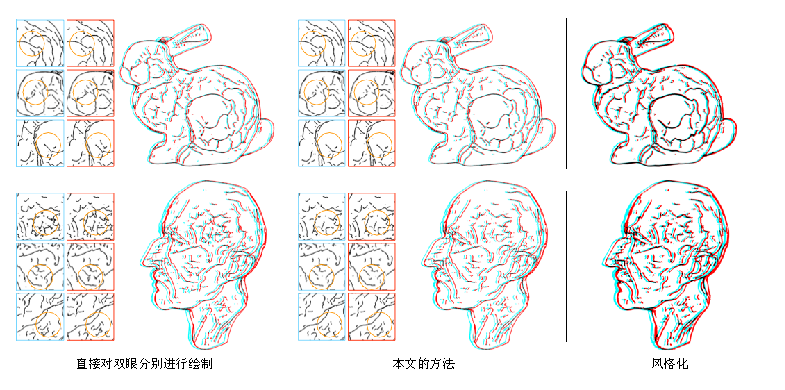
\includegraphics[width=1.2\linewidth]{basic}}
    \caption[与直接方法的双目图像的对比]{\label{fig:basic}
    用直接方法生成的双目图像和用本文提出的方法生成的双目图像的对比。从左到右分别是分别对左右两眼进行绘制、使用本文的方法得到的\stc{}的结果以及\stc{}结果上进行进一步风格化的结果。使用的三维模型来自DeCarlo等人的工作\cite{DFRS03}。
    }
\end{figure}
  
\begin{figure}[tbh]
    \centering
    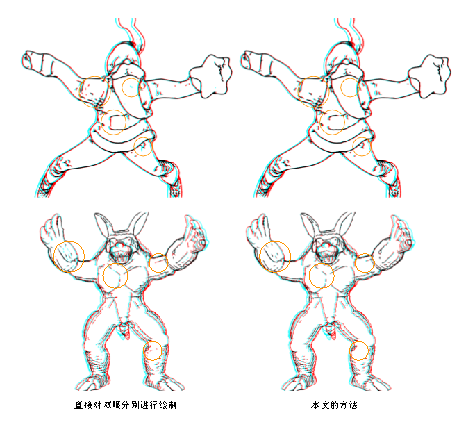
\includegraphics[width=\linewidth]{more}
    \caption[更多与直接方法的双目图像的对比]{\label{fig:more}
    更多用直接方法生成的双目图像和用本文提出的方法生成的双目图像的对比。
    }
\end{figure}

首先,为了评估本文提出的方法的质量,本文展示了用直接方法生成的双目图像和用本文提出的方法生成的双目图像的对比(\autoref{fig:basic}, \autoref{fig:more})。图中有部分放大的区域,从这些区域可以看出更细节的对比。从这些结果可以看出,本文提出的方法有效地消除了不是\stc{}那些\con{}和\scon{}。

\begin{figure}[tbh]
    \centering
    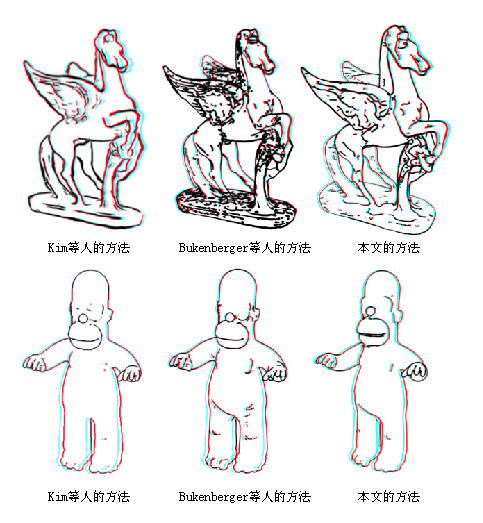
\includegraphics[width=0.8\linewidth]{comparison}
    \caption[与前人工作的双目图像的对比]{\label{fig:comparison}
    前人工作\cite{kim2013stereoscopic,bukenberger2018stereo}所展示的结果和本文方法所生成的结果的对比。由于无法获取前人工作所展示结果使用的一些绘制参数,所以本文方法生成的结果是通过手动调节参数来尽量使得艺术效果上尽量一致。但是由于使用的模型或者\con{}和\scon{}绘制算法实现上的差异,部分细节仍会有所出入。天马的图像是根据深度对笔画宽度进行风格化的结果。使用的模型来自IMATI和CNR的AIM@SHAPE-VISIONAIR Shape Repository\cite{INR04}。}
\end{figure}  

其次,为了进一步验证本文提出的方法的有效性,本文在\autoref{fig:comparison}中展示了前人工作\cite{kim2013stereoscopic,bukenberger2018stereo}所展示的结果和本文方法所生成的结果的对比。由于无法获取前人工作所展示的结果使用的一些绘制参数,所以本文方法生成的结果是通过手动调节参数来尽量使得艺术效果上尽量一致。从这些结果可以看出,尽管细节上有些许差异,本文提出的方法能够实现的\stcy{}效果与前人方法所实现的效果基本一致。

\begin{figure}[tbh]
    \centering
    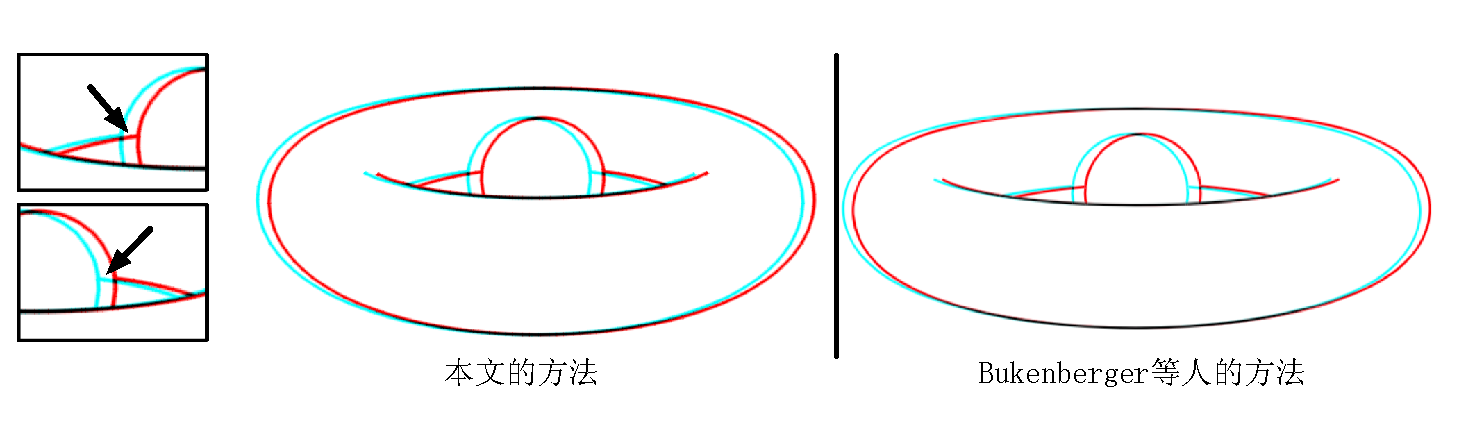
\includegraphics[width=\linewidth]{hidden}
    \caption[遮挡情况下的匹配]{\label{fig:hidden}
    在线条被遮挡的情况下的匹配。使用了方框和箭头来指出被遮挡的线条。右边展示了来自于另一工作\cite{bukenberger2018stereo}的相似结果作为对比。}
\end{figure}

尽管本文提出的方法只在图像空间进行处理,但是被遮挡的线条也无须任何特别处理就能被正确地匹配,因为被遮挡的轮廓点也被存储在了\ppll{}之中。\autoref{fig:hidden}展示了一个在存在遮挡的情况下用本文设计的方法生成的和前人工作中的结果相似的的结果。

由于本文提出的方法不依赖于任何的预计算,所以本文提出的方法支持变化视点下的动态场景,并且支持实时的参数调节。

\section{效率对比}

\begin{table}[tbh]
    \renewcommand{\arraystretch}{1.3}
    \centering
  \begin{threeparttable}
    \caption[示例场景的效率数据]{示例场景的效率数据$^1$}
    \label{tab:performance}
    %\scriptsize
    % \small
    \centering
    \begin{tabular}{c|cc|ccc|c}
    \hline
    \multirow{2}{*}{场景} & \multirow{2}{*}{顶点数} & \multirow{2}{*}{面片数} & \multicolumn{4}{c}{效率 (ms / FPS)} \\
    \cline{4-7}
    & & & I & II & III & Total \\
    \hline
    Bunny (\autoref{fig:basic}) & 35947 & 69451 & {2.2} & {2.1} & {0.3} & {4.9/204.0} \\
    Max Planck (\autoref{fig:basic}) & 49132 & 98260 & {2.5} & {3.0} & {0.5} & {6.3/158.7} \\
    Homer (\autoref{fig:comparison}) & 5103 & 10202 & {0.6} & {2.3} & {0.1} & {3.2/312.5} \\
    Pegasus (\autoref{fig:comparison}) & 63544 & 127095 & {3.7} & {2.7} & {0.7} & {7.4/135.1} \\
    \hline
    \end{tabular}
    \begin{tablenotes}
      \item $^1$ 从左到右分别是:场景,顶点数,面片数以及阶段I,阶段II,阶段III以及整体的效率数据。数据是在没有启用线条风格化的情况下记录的。
    \end{tablenotes}
  \end{threeparttable}
\end{table}

本文使用PC平台上的OpenGL 4.6实现所展示的\stc{}\vdl{}绘制系统,所使用的CPU为Intel Xeon E3,GPU为NVIDIA GeForce RTX 2080 Ti。绘制图像的分辨率为1024$\times$768。

\autoref{tab:performance}展示了绘制\autoref{fig:basic}和\autoref{fig:comparison}所示结果的效率。需要指出的是,这些时间数据是在没有启用线条风格化的情况下记录的。在对比之下可以看出,Kim等人实现的系统\cite{kim2013stereoscopic}在使用GPU并且顶点数量达到30,000的情况下效率是每秒3帧。Bukenberger等人在他们的工作中实现了一个更高效的系统\cite{bukenberger2018stereo},在使用CPU并且面片数达到20,000的情况下能够达到每秒24帧的效率,但是在他们的工作中没有提及使用GPU的情况。然而,这样的效率是他们在没有正确考虑视点相关的遮挡的情况下得到的。在他们的方法中,即使对于像犹他茶壶(Utah Teapot)这样只有2464面片的小模型,完整考虑视点相关遮挡所需要的视图算法也需要消耗0.25秒,而对于像斯坦福兔子(Stanford Bunny)这样较大的模型则需要将近5秒。与上述前人的方法相比,本文提出的方法能够以更高的效率实现正确的\stc{}\vdl{}绘制。
\chapter{总结与展望}

\section{全文总结}

线绘制是一种表现物体外形的重要技术。按照视点相关性,线绘制技术中探讨的线条可以分为视点相关线和视点无关线。其中,\con{}和\scon{}都属于视点相关线,如果这类线条不以立体一致的方式进行绘制,将会给用户带来不适。针对\vdl{}在双目绘制下出现的问题,本文先是介绍了\vdl{}和双目绘制的概念,然后对前人提出的对极滑动性的概念和立体一致的\vdl{}的绘制方法进行了说明。接着,在前人工作的基础上,本文提出了一种\stc{}\vdl{}的实时绘制方法,该方法的核心想法在于通过一个图像空间的搜索来完成\vdp{}的\epsl{}的判定,而不是像之前的工作中那样对多个视点进行采样来完成\epsl{}判定。具体地,本文拓展了\epsl{}的概念并推导了一个新的\epsl{}的判定方法:通过\vdp{}的对应视点的轨迹的单调性来判定\epsl{}。在这个推导的基础上,本文提出了一个多阶段的绘制算法,该算法首先计算出\vdl{}以及轨迹函数的极值点与区间端点,然后根据这些信息在图像空间完成\epsl{}的判定。本文提出的算法同时支持\con{}以及\scon{},并且支持进一步的风格化绘制。对于\con{}和\scon{}以外的\vdl{},也可以通过同样的过程进行推导,并在同样的算法框架下完成\stc{}的绘制。实验结果表明,本文提出的方法在正确地消去非\stc{}\vdl{}的同时高质量地保留了\stc{}\epsl{}。本文提出的算法对GPU十分友好,其中所有步骤都可以在着色器中实现。由于本文提出的算法是完全以每一帧的信息作为输入进行计算的,不依赖于任何预计算的信息,而且效率很高,所以能够让用户实时地调整三维模型并且对各种绘制参数进行调整。

\section{未来展望}

尽管本文提出的方法能够实现实时的\stc{}\vdl{}绘制,但还该方法还存在一些限制。首先,对于错误匹配的处理还不够完善。在错误匹配来自于同一个物体时,使用物体的索引来排除错误匹配的方法会失效。一个更可靠的用于排除错误匹配的方法还有待开发。其次,在本文的讨论中还没有对\vdl{}的时序一致性进行考虑。换言之,每帧绘制的\vdl{}在时间上可能会不够连续,因此在视频中会出现\vdl{}的闪烁。在启用线条风格化的情况下,这种闪烁的情况会更加明显。出现这个问题的根源在于立体一致性和时序一致性之间会存在冲突,如果想要保证立体一致性,则需要根据物体的几何特征进行线条的风格化,而如果想要保证时序一致性,那么需要传递风格化参数,二者如何平衡是一个很难解决的问题。因此,设计出一个能够支持时序一致性的方法来完成\stc{}\vdl{}的绘制,是一个很有价值的研究方向。


\ZJUbackmatter
%%%%%%%%%%%%%%%%%%%%%%%%%%%%%%
%% 参考文献
%%%%%%%%%%%%%%%%%%%%%%%%%%%%%%
% \ZJUthesisbib{thesisbib}
\printbibliography[title={参考文献}]

%%%%%%%%%%%%%%%%%%%%%%%%%%%%%%
%% 发表论文目录
%%%%%%%%%%%%%%%%%%%%%%%%%%%%%%
\begin{publications}
\begin{enumerate}[label={[\arabic*]}]
% \item 猪八戒,猪悟能,天蓬元帅,等. 论流体食物的持久保存 [D]. 硕士学位论文. 北京: 广寒宫大学, 2005
\item Dejing He, Rui Wang, Hujun Bao. Real-Time Rendering of Stereo-Consistent, 2019 IEEE Conference on Virtual Reality and 3D User Interfaces[C]. [S.l. : s.n.], 2019:81-87.
\end{enumerate}

\end{publications}


%%%%%%%%%%%%%%%%%%%%%%%%%%%%%%
%% 致谢页
%%%%%%%%%%%%%%%%%%%%%%%%%%%%%%
\begin{thanks}

% 感谢我的导师王锐教授在研究生期间对我的指导,让我在计算机图形学领域收获了丰富的学识和经验。这两年多时间的学习必定会让我受益终生。

% 感谢实验室各位同学们在研究生期间对我的帮助和鼓励。无论是科研上还是生活上,和你们相伴的时光十分愉快。与这么优秀的同学共事,是我的荣幸。

% 最后感谢家人对我默默的支持,有了你们的支持我才能在人生道路上不折不挠、奋勇前进。

% \begin{flushright}
% {
%   \large{何淂劲}\hspace{0.5in}

%   \large{二零二零年三月}\hspace{0.18in}
% }

% \end{flushright}

\end{thanks}



\end{document}
